% Options for packages loaded elsewhere
\PassOptionsToPackage{unicode}{hyperref}
\PassOptionsToPackage{hyphens}{url}
\PassOptionsToPackage{dvipsnames,svgnames,x11names}{xcolor}
%
\documentclass[
  letterpaper,
  DIV=11,
  numbers=noendperiod]{scrartcl}

\usepackage{amsmath,amssymb}
\usepackage{lmodern}
\usepackage{iftex}
\ifPDFTeX
  \usepackage[T1]{fontenc}
  \usepackage[utf8]{inputenc}
  \usepackage{textcomp} % provide euro and other symbols
\else % if luatex or xetex
  \usepackage{unicode-math}
  \defaultfontfeatures{Scale=MatchLowercase}
  \defaultfontfeatures[\rmfamily]{Ligatures=TeX,Scale=1}
\fi
% Use upquote if available, for straight quotes in verbatim environments
\IfFileExists{upquote.sty}{\usepackage{upquote}}{}
\IfFileExists{microtype.sty}{% use microtype if available
  \usepackage[]{microtype}
  \UseMicrotypeSet[protrusion]{basicmath} % disable protrusion for tt fonts
}{}
\makeatletter
\@ifundefined{KOMAClassName}{% if non-KOMA class
  \IfFileExists{parskip.sty}{%
    \usepackage{parskip}
  }{% else
    \setlength{\parindent}{0pt}
    \setlength{\parskip}{6pt plus 2pt minus 1pt}}
}{% if KOMA class
  \KOMAoptions{parskip=half}}
\makeatother
\usepackage{xcolor}
\setlength{\emergencystretch}{3em} % prevent overfull lines
\setcounter{secnumdepth}{-\maxdimen} % remove section numbering
% Make \paragraph and \subparagraph free-standing
\ifx\paragraph\undefined\else
  \let\oldparagraph\paragraph
  \renewcommand{\paragraph}[1]{\oldparagraph{#1}\mbox{}}
\fi
\ifx\subparagraph\undefined\else
  \let\oldsubparagraph\subparagraph
  \renewcommand{\subparagraph}[1]{\oldsubparagraph{#1}\mbox{}}
\fi

\usepackage{color}
\usepackage{fancyvrb}
\newcommand{\VerbBar}{|}
\newcommand{\VERB}{\Verb[commandchars=\\\{\}]}
\DefineVerbatimEnvironment{Highlighting}{Verbatim}{commandchars=\\\{\}}
% Add ',fontsize=\small' for more characters per line
\usepackage{framed}
\definecolor{shadecolor}{RGB}{241,243,245}
\newenvironment{Shaded}{\begin{snugshade}}{\end{snugshade}}
\newcommand{\AlertTok}[1]{\textcolor[rgb]{0.68,0.00,0.00}{#1}}
\newcommand{\AnnotationTok}[1]{\textcolor[rgb]{0.37,0.37,0.37}{#1}}
\newcommand{\AttributeTok}[1]{\textcolor[rgb]{0.40,0.45,0.13}{#1}}
\newcommand{\BaseNTok}[1]{\textcolor[rgb]{0.68,0.00,0.00}{#1}}
\newcommand{\BuiltInTok}[1]{\textcolor[rgb]{0.00,0.23,0.31}{#1}}
\newcommand{\CharTok}[1]{\textcolor[rgb]{0.13,0.47,0.30}{#1}}
\newcommand{\CommentTok}[1]{\textcolor[rgb]{0.37,0.37,0.37}{#1}}
\newcommand{\CommentVarTok}[1]{\textcolor[rgb]{0.37,0.37,0.37}{\textit{#1}}}
\newcommand{\ConstantTok}[1]{\textcolor[rgb]{0.56,0.35,0.01}{#1}}
\newcommand{\ControlFlowTok}[1]{\textcolor[rgb]{0.00,0.23,0.31}{#1}}
\newcommand{\DataTypeTok}[1]{\textcolor[rgb]{0.68,0.00,0.00}{#1}}
\newcommand{\DecValTok}[1]{\textcolor[rgb]{0.68,0.00,0.00}{#1}}
\newcommand{\DocumentationTok}[1]{\textcolor[rgb]{0.37,0.37,0.37}{\textit{#1}}}
\newcommand{\ErrorTok}[1]{\textcolor[rgb]{0.68,0.00,0.00}{#1}}
\newcommand{\ExtensionTok}[1]{\textcolor[rgb]{0.00,0.23,0.31}{#1}}
\newcommand{\FloatTok}[1]{\textcolor[rgb]{0.68,0.00,0.00}{#1}}
\newcommand{\FunctionTok}[1]{\textcolor[rgb]{0.28,0.35,0.67}{#1}}
\newcommand{\ImportTok}[1]{\textcolor[rgb]{0.00,0.46,0.62}{#1}}
\newcommand{\InformationTok}[1]{\textcolor[rgb]{0.37,0.37,0.37}{#1}}
\newcommand{\KeywordTok}[1]{\textcolor[rgb]{0.00,0.23,0.31}{#1}}
\newcommand{\NormalTok}[1]{\textcolor[rgb]{0.00,0.23,0.31}{#1}}
\newcommand{\OperatorTok}[1]{\textcolor[rgb]{0.37,0.37,0.37}{#1}}
\newcommand{\OtherTok}[1]{\textcolor[rgb]{0.00,0.23,0.31}{#1}}
\newcommand{\PreprocessorTok}[1]{\textcolor[rgb]{0.68,0.00,0.00}{#1}}
\newcommand{\RegionMarkerTok}[1]{\textcolor[rgb]{0.00,0.23,0.31}{#1}}
\newcommand{\SpecialCharTok}[1]{\textcolor[rgb]{0.37,0.37,0.37}{#1}}
\newcommand{\SpecialStringTok}[1]{\textcolor[rgb]{0.13,0.47,0.30}{#1}}
\newcommand{\StringTok}[1]{\textcolor[rgb]{0.13,0.47,0.30}{#1}}
\newcommand{\VariableTok}[1]{\textcolor[rgb]{0.07,0.07,0.07}{#1}}
\newcommand{\VerbatimStringTok}[1]{\textcolor[rgb]{0.13,0.47,0.30}{#1}}
\newcommand{\WarningTok}[1]{\textcolor[rgb]{0.37,0.37,0.37}{\textit{#1}}}

\providecommand{\tightlist}{%
  \setlength{\itemsep}{0pt}\setlength{\parskip}{0pt}}\usepackage{longtable,booktabs,array}
\usepackage{calc} % for calculating minipage widths
% Correct order of tables after \paragraph or \subparagraph
\usepackage{etoolbox}
\makeatletter
\patchcmd\longtable{\par}{\if@noskipsec\mbox{}\fi\par}{}{}
\makeatother
% Allow footnotes in longtable head/foot
\IfFileExists{footnotehyper.sty}{\usepackage{footnotehyper}}{\usepackage{footnote}}
\makesavenoteenv{longtable}
\usepackage{graphicx}
\makeatletter
\def\maxwidth{\ifdim\Gin@nat@width>\linewidth\linewidth\else\Gin@nat@width\fi}
\def\maxheight{\ifdim\Gin@nat@height>\textheight\textheight\else\Gin@nat@height\fi}
\makeatother
% Scale images if necessary, so that they will not overflow the page
% margins by default, and it is still possible to overwrite the defaults
% using explicit options in \includegraphics[width, height, ...]{}
\setkeys{Gin}{width=\maxwidth,height=\maxheight,keepaspectratio}
% Set default figure placement to htbp
\makeatletter
\def\fps@figure{htbp}
\makeatother

\KOMAoption{captions}{tableheading}
\makeatletter
\makeatother
\makeatletter
\makeatother
\makeatletter
\@ifpackageloaded{caption}{}{\usepackage{caption}}
\AtBeginDocument{%
\ifdefined\contentsname
  \renewcommand*\contentsname{Table of contents}
\else
  \newcommand\contentsname{Table of contents}
\fi
\ifdefined\listfigurename
  \renewcommand*\listfigurename{List of Figures}
\else
  \newcommand\listfigurename{List of Figures}
\fi
\ifdefined\listtablename
  \renewcommand*\listtablename{List of Tables}
\else
  \newcommand\listtablename{List of Tables}
\fi
\ifdefined\figurename
  \renewcommand*\figurename{Figure}
\else
  \newcommand\figurename{Figure}
\fi
\ifdefined\tablename
  \renewcommand*\tablename{Table}
\else
  \newcommand\tablename{Table}
\fi
}
\@ifpackageloaded{float}{}{\usepackage{float}}
\floatstyle{ruled}
\@ifundefined{c@chapter}{\newfloat{codelisting}{h}{lop}}{\newfloat{codelisting}{h}{lop}[chapter]}
\floatname{codelisting}{Listing}
\newcommand*\listoflistings{\listof{codelisting}{List of Listings}}
\makeatother
\makeatletter
\@ifpackageloaded{caption}{}{\usepackage{caption}}
\@ifpackageloaded{subcaption}{}{\usepackage{subcaption}}
\makeatother
\makeatletter
\@ifpackageloaded{tcolorbox}{}{\usepackage[many]{tcolorbox}}
\makeatother
\makeatletter
\@ifundefined{shadecolor}{\definecolor{shadecolor}{rgb}{.97, .97, .97}}
\makeatother
\makeatletter
\makeatother
\ifLuaTeX
  \usepackage{selnolig}  % disable illegal ligatures
\fi
\IfFileExists{bookmark.sty}{\usepackage{bookmark}}{\usepackage{hyperref}}
\IfFileExists{xurl.sty}{\usepackage{xurl}}{} % add URL line breaks if available
\urlstyle{same} % disable monospaced font for URLs
\hypersetup{
  pdftitle={Presentation: Communicating data and code},
  pdfauthor={Thomas H. Simm},
  colorlinks=true,
  linkcolor={blue},
  filecolor={Maroon},
  citecolor={Blue},
  urlcolor={Blue},
  pdfcreator={LaTeX via pandoc}}

\title{Presentation: Communicating data and code}
\usepackage{etoolbox}
\makeatletter
\providecommand{\subtitle}[1]{% add subtitle to \maketitle
  \apptocmd{\@title}{\par {\large #1 \par}}{}{}
}
\makeatother
\subtitle{Using the notebook format and app frameworks to communicate
code and data}
\author{Thomas H. Simm}
\date{}

\begin{document}
\maketitle
\ifdefined\Shaded\renewenvironment{Shaded}{\begin{tcolorbox}[enhanced, boxrule=0pt, interior hidden, breakable, frame hidden, borderline west={3pt}{0pt}{shadecolor}, sharp corners]}{\end{tcolorbox}}\fi

\hypertarget{content}{%
\subsection{Content}\label{content}}

\begin{itemize}
\tightlist
\item
  Notebooks

  \begin{itemize}
  \tightlist
  \item
    What are they?
  \item
    Examples
  \item
    Pros and cons
  \end{itemize}
\item
  Streamlit

  \begin{itemize}
  \tightlist
  \item
    Use in communicating code
  \end{itemize}
\item
  Websites and HTML

  \begin{itemize}
  \tightlist
  \item
    Converting notebooks to HTML and websites
  \end{itemize}
\item
  Presentations

  \begin{itemize}
  \tightlist
  \item
    Using notebooks for presentations
  \end{itemize}
\item
  Tabular Data

  \begin{itemize}
  \tightlist
  \item
    Comments on Excel
  \item
    Thoughts on code alternatives
  \end{itemize}
\end{itemize}

\hypertarget{overview-communicating-code}{%
\section{Overview Communicating
code}\label{overview-communicating-code}}

\begin{itemize}
\item
  Communicating when code is a large element of what is being presented

  \begin{itemize}
  \tightlist
  \item
    Microsoft Word/ppt- type methods aren't set-up well to include code
  \item
    Programming files (e.g.~\texttt{.py}) aren't set-up well to share or
    understand what is going on in the code
  \item
    Videoing code with outputs is an option, but doesn't translate to
    other formats (i.e.~we may also need to do a written format of this)
  \item
    Excel is a good way to present tabular data \textbf{but} if we are
    only viewing is slow and inefficient
  \end{itemize}
\item
  Better ways?

  \begin{itemize}
  \tightlist
  \item
    Programming notebooks (e.g.\texttt{.ipynb}) offer a good and easy to
    share code alongside written content

    \begin{itemize}
    \tightlist
    \item
      And can be converted to other formats easily such as html
    \end{itemize}
  \item
    Apps (e.g.~streamlit) can be good

    \begin{itemize}
    \tightlist
    \item
      particularly when interactivity is required
    \end{itemize}
  \end{itemize}
\end{itemize}

\hypertarget{notebooks-general}{%
\section{Notebooks General}\label{notebooks-general}}

\hypertarget{jupyter-notebooks}{%
\subsection{Jupyter Notebooks}\label{jupyter-notebooks}}

From
\href{https://talkpython.fm/episodes/show/394/awesome-jupyter-libraries-and-extensions-in-2022}{TalkPython:
Awesome Jupyter Libraries and Extensions}

\begin{quote}
Jupyter is an amazing environment for exploring data and generating
executable reports with Python. But there are many external tools,
extensions, and libraries to make it so much better and make you more
productive.
\end{quote}

\begin{itemize}
\tightlist
\item
  A notebook consists of two parts

  \begin{itemize}
  \tightlist
  \item
    markdown part where we can:

    \begin{itemize}
    \tightlist
    \item
      write text, add images, links, html, LaTeX etc
    \end{itemize}
  \item
    code part which runs and displays output of code
  \end{itemize}
\end{itemize}

Some links:

\begin{itemize}
\tightlist
\item
  \href{https://jupyterbook.org/en/stable/intro.html}{Jupyter Book}
\item
  \href{https://github.com/markusschanta/awesome-jupyter}{A curated list
  of awesome Jupyter projects}
\item
  \href{https://best-practice-and-impact.github.io/qa-of-code-guidance/code_documentation.html\#generating-html-documentation}{Code
  Documentation QA of Code}
\item
  \href{https://www.fast.ai/posts/2019-05-13-blogging-advice.html}{FastAI
  guide for better blogs}
\end{itemize}

\hypertarget{example-of-a-notebook}{%
\subsection{Example of a notebook}\label{example-of-a-notebook}}

An example notebook

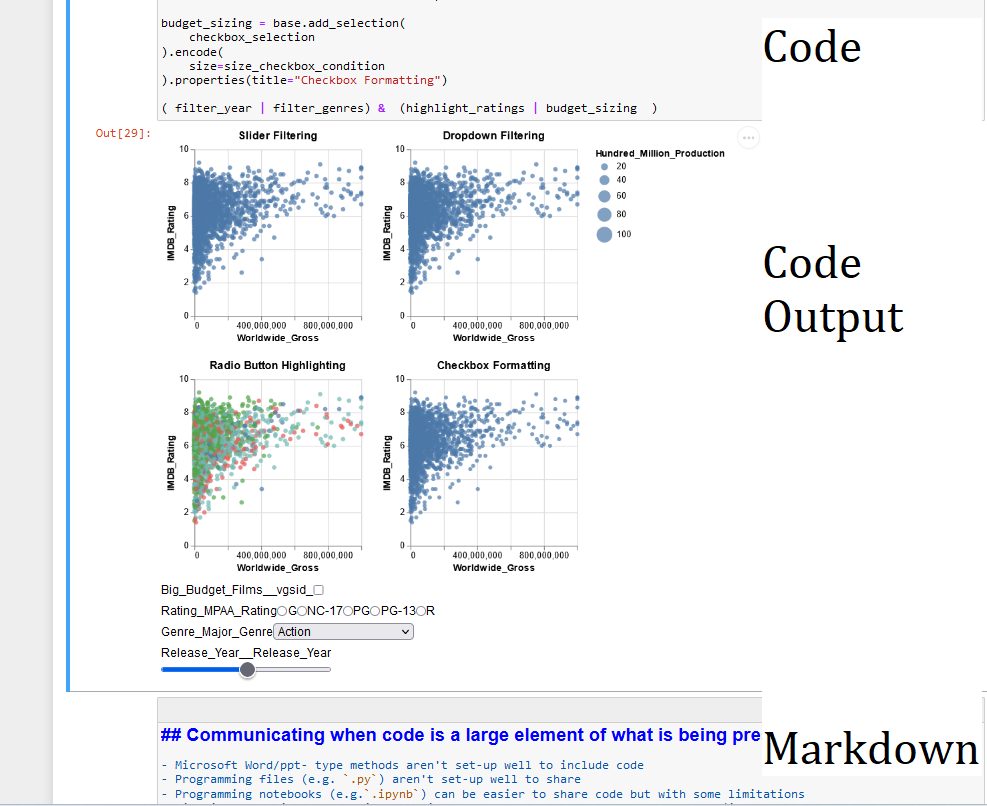
\includegraphics{ghtop_images/jupyter.png}

\hypertarget{markdown-in-a-notebook-1}{%
\subsection{Markdown in a notebook 1}\label{markdown-in-a-notebook-1}}

Some useful commands:

\begin{enumerate}
\def\labelenumi{\arabic{enumi}.}
\item
  \texttt{\#\ Notebooks\ Markdown\ and\ Code} and
  \texttt{\#\#\ Markdown\ in\ a\ notebook}
\item
  \texttt{!{[}{]}(ghtop\_images/pest.png)} looks like this
\end{enumerate}

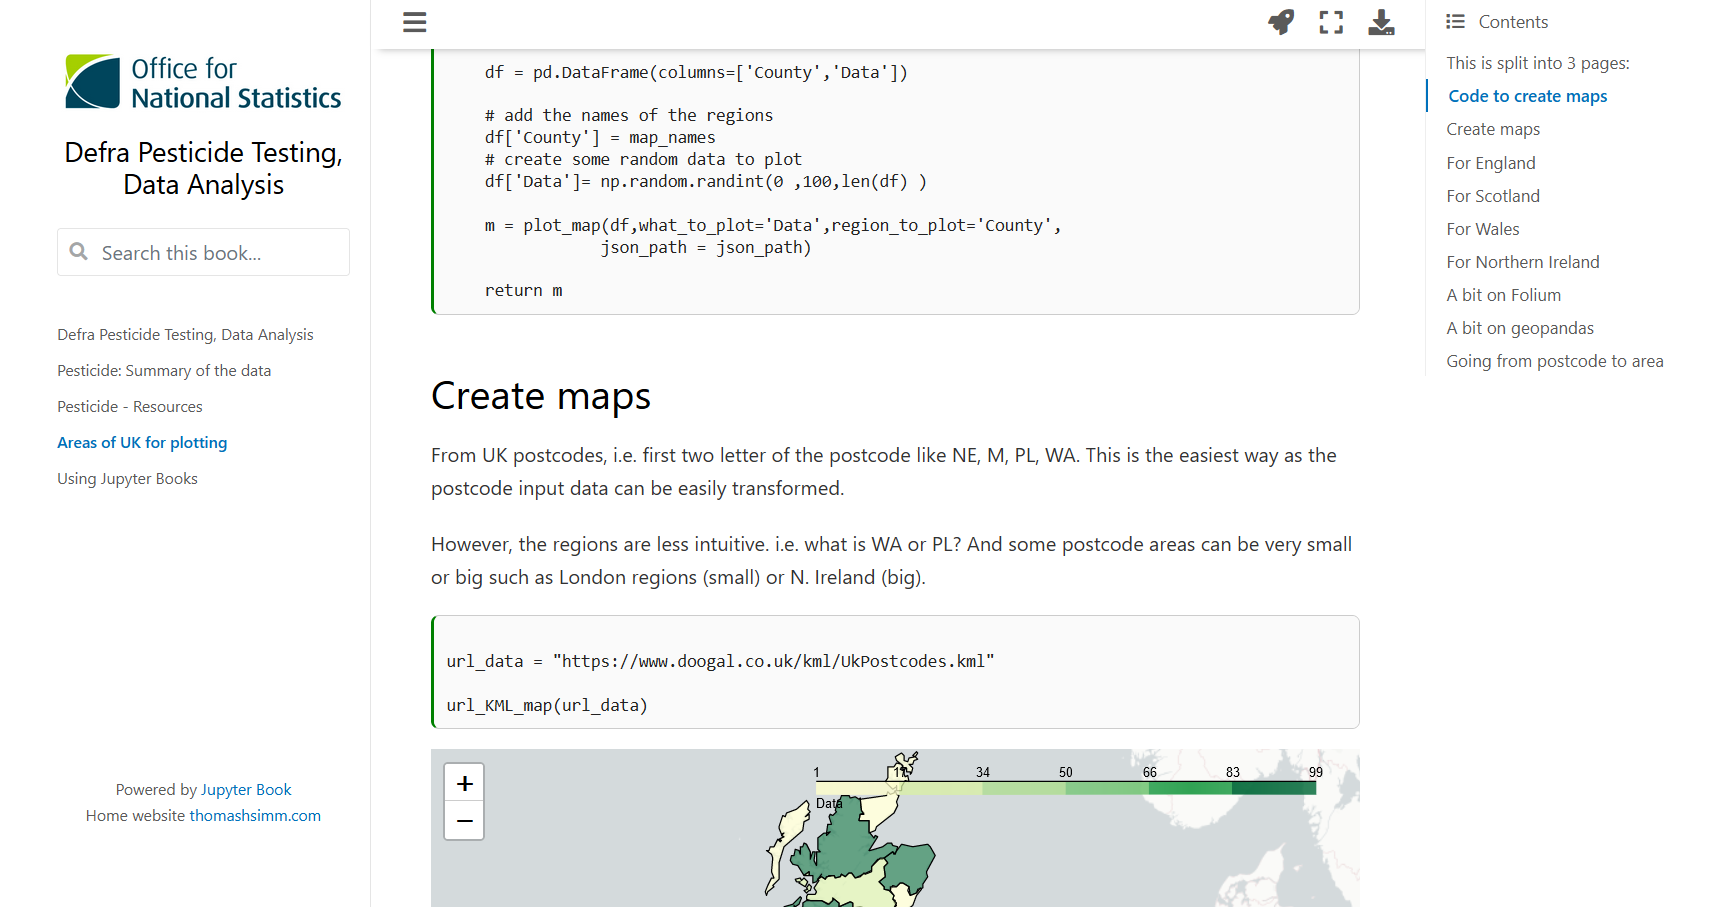
\includegraphics{ghtop_images/pest.png}

\hypertarget{markdown-in-a-notebook-2}{%
\subsection{Markdown in a notebook 2}\label{markdown-in-a-notebook-2}}

\begin{enumerate}
\def\labelenumi{\arabic{enumi}.}
\setcounter{enumi}{2}
\tightlist
\item
  And the same with a mp4 file
  \texttt{!{[}{]}(ghtop\_images/revealjs.mp4)}
\end{enumerate}

\hypertarget{markdown-in-a-notebook-3}{%
\subsection{Markdown in a notebook 3}\label{markdown-in-a-notebook-3}}

\begin{enumerate}
\def\labelenumi{\arabic{enumi}.}
\setcounter{enumi}{3}
\tightlist
\item
  \texttt{\textgreater{}\ If\ we\ want\ text\ like\ this}
\end{enumerate}

\begin{quote}
If we want text like this
\end{quote}

\begin{enumerate}
\def\labelenumi{\arabic{enumi}.}
\setcounter{enumi}{4}
\tightlist
\item
  Or if we want code use `a = b + c`
\end{enumerate}

or:

```

a = b

a = a + c

```

\begin{verbatim}

a = b

a = a + c
\end{verbatim}

\hypertarget{markdown-in-a-notebook-4}{%
\subsection{Markdown in a notebook 4}\label{markdown-in-a-notebook-4}}

\begin{enumerate}
\def\labelenumi{\arabic{enumi}.}
\setcounter{enumi}{5}
\tightlist
\item
  HTML works too
\end{enumerate}

\begin{verbatim}
<img src="ghtop_images/pest.png"></img>
\end{verbatim}

\hypertarget{code-in-a-notebook}{%
\subsection{Code in a notebook}\label{code-in-a-notebook}}

Example interactive format using altair:

\begin{Shaded}
\begin{Highlighting}[]
\ImportTok{import}\NormalTok{ altair }\ImportTok{as}\NormalTok{ alt}
\ImportTok{from}\NormalTok{ vega\_datasets }\ImportTok{import}\NormalTok{ data}

\NormalTok{movies }\OperatorTok{=}\NormalTok{ alt.UrlData(}
\NormalTok{    data.movies.url,}
    \BuiltInTok{format}\OperatorTok{=}\NormalTok{alt.DataFormat(parse}\OperatorTok{=}\NormalTok{\{}\StringTok{"Release\_Date"}\NormalTok{:}\StringTok{"date"}\NormalTok{\})}
\NormalTok{)}
\NormalTok{ratings }\OperatorTok{=}\NormalTok{ [}\StringTok{\textquotesingle{}G\textquotesingle{}}\NormalTok{, }\StringTok{\textquotesingle{}NC{-}17\textquotesingle{}}\NormalTok{, }\StringTok{\textquotesingle{}PG\textquotesingle{}}\NormalTok{, }\StringTok{\textquotesingle{}PG{-}13\textquotesingle{}}\NormalTok{, }\StringTok{\textquotesingle{}R\textquotesingle{}}\NormalTok{]}
\NormalTok{genres }\OperatorTok{=}\NormalTok{ [}\StringTok{\textquotesingle{}Action\textquotesingle{}}\NormalTok{, }\StringTok{\textquotesingle{}Adventure\textquotesingle{}}\NormalTok{, }\StringTok{\textquotesingle{}Black Comedy\textquotesingle{}}\NormalTok{, }\StringTok{\textquotesingle{}Comedy\textquotesingle{}}\NormalTok{,}
       \StringTok{\textquotesingle{}Concert/Performance\textquotesingle{}}\NormalTok{, }\StringTok{\textquotesingle{}Documentary\textquotesingle{}}\NormalTok{, }\StringTok{\textquotesingle{}Drama\textquotesingle{}}\NormalTok{, }\StringTok{\textquotesingle{}Horror\textquotesingle{}}\NormalTok{, }\StringTok{\textquotesingle{}Musical\textquotesingle{}}\NormalTok{,}
       \StringTok{\textquotesingle{}Romantic Comedy\textquotesingle{}}\NormalTok{, }\StringTok{\textquotesingle{}Thriller/Suspense\textquotesingle{}}\NormalTok{, }\StringTok{\textquotesingle{}Western\textquotesingle{}}\NormalTok{]}

\NormalTok{base }\OperatorTok{=}\NormalTok{ alt.Chart(movies, width}\OperatorTok{=}\DecValTok{200}\NormalTok{, height}\OperatorTok{=}\DecValTok{200}\NormalTok{).mark\_point(filled}\OperatorTok{=}\VariableTok{True}\NormalTok{).transform\_calculate(}
\NormalTok{    Rounded\_IMDB\_Rating }\OperatorTok{=} \StringTok{"floor(datum.IMDB\_Rating)"}\NormalTok{,}
\NormalTok{    Hundred\_Million\_Production }\OperatorTok{=}  \StringTok{"datum.Production\_Budget \textgreater{} 100000000.0 ? 100 : 10"}\NormalTok{,}
\NormalTok{    Release\_Year }\OperatorTok{=} \StringTok{"year(datum.Release\_Date)"}
\NormalTok{).transform\_filter(}
\NormalTok{    alt.datum.IMDB\_Rating }\OperatorTok{\textgreater{}} \DecValTok{0}
\NormalTok{).transform\_filter(}
\NormalTok{    alt.FieldOneOfPredicate(field}\OperatorTok{=}\StringTok{\textquotesingle{}MPAA\_Rating\textquotesingle{}}\NormalTok{, oneOf}\OperatorTok{=}\NormalTok{ratings)}
\NormalTok{).encode(}
\NormalTok{    x}\OperatorTok{=}\NormalTok{alt.X(}\StringTok{\textquotesingle{}Worldwide\_Gross:Q\textquotesingle{}}\NormalTok{, scale}\OperatorTok{=}\NormalTok{alt.Scale(domain}\OperatorTok{=}\NormalTok{(}\DecValTok{100000}\NormalTok{,}\DecValTok{10}\OperatorTok{**}\DecValTok{9}\NormalTok{), clamp}\OperatorTok{=}\VariableTok{True}\NormalTok{)),}
\NormalTok{    y}\OperatorTok{=}\StringTok{\textquotesingle{}IMDB\_Rating:Q\textquotesingle{}}\NormalTok{,}
\NormalTok{    tooltip}\OperatorTok{=}\StringTok{"Title:N"}
\NormalTok{)}

\CommentTok{\# A slider filter}
\NormalTok{year\_slider }\OperatorTok{=}\NormalTok{ alt.binding\_range(}\BuiltInTok{min}\OperatorTok{=}\DecValTok{1969}\NormalTok{, }\BuiltInTok{max}\OperatorTok{=}\DecValTok{2018}\NormalTok{, step}\OperatorTok{=}\DecValTok{1}\NormalTok{)}
\NormalTok{slider\_selection }\OperatorTok{=}\NormalTok{ alt.selection\_single(bind}\OperatorTok{=}\NormalTok{year\_slider, fields}\OperatorTok{=}\NormalTok{[}\StringTok{\textquotesingle{}Release\_Year\textquotesingle{}}\NormalTok{], name}\OperatorTok{=}\StringTok{"Release Year\_"}\NormalTok{)}


\NormalTok{filter\_year }\OperatorTok{=}\NormalTok{ base.add\_selection(}
\NormalTok{    slider\_selection}
\NormalTok{).transform\_filter(}
\NormalTok{    slider\_selection}
\NormalTok{).properties(title}\OperatorTok{=}\StringTok{"Slider Filtering"}\NormalTok{)}

\CommentTok{\# A dropdown filter}
\NormalTok{genre\_dropdown }\OperatorTok{=}\NormalTok{ alt.binding\_select(options}\OperatorTok{=}\NormalTok{genres)}
\NormalTok{genre\_select }\OperatorTok{=}\NormalTok{ alt.selection\_single(fields}\OperatorTok{=}\NormalTok{[}\StringTok{\textquotesingle{}Major\_Genre\textquotesingle{}}\NormalTok{], bind}\OperatorTok{=}\NormalTok{genre\_dropdown, name}\OperatorTok{=}\StringTok{"Genre"}\NormalTok{)}

\NormalTok{filter\_genres }\OperatorTok{=}\NormalTok{ base.add\_selection(}
\NormalTok{    genre\_select}
\NormalTok{).transform\_filter(}
\NormalTok{    genre\_select}
\NormalTok{).properties(title}\OperatorTok{=}\StringTok{"Dropdown Filtering"}\NormalTok{)}

\CommentTok{\#color changing marks}
\NormalTok{rating\_radio }\OperatorTok{=}\NormalTok{ alt.binding\_radio(options}\OperatorTok{=}\NormalTok{ratings)}

\NormalTok{rating\_select }\OperatorTok{=}\NormalTok{ alt.selection\_single(fields}\OperatorTok{=}\NormalTok{[}\StringTok{\textquotesingle{}MPAA\_Rating\textquotesingle{}}\NormalTok{], bind}\OperatorTok{=}\NormalTok{rating\_radio, name}\OperatorTok{=}\StringTok{"Rating"}\NormalTok{)}
\NormalTok{rating\_color\_condition }\OperatorTok{=}\NormalTok{ alt.condition(rating\_select,}
\NormalTok{                      alt.Color(}\StringTok{\textquotesingle{}MPAA\_Rating:N\textquotesingle{}}\NormalTok{, legend}\OperatorTok{=}\VariableTok{None}\NormalTok{),}
\NormalTok{                      alt.value(}\StringTok{\textquotesingle{}lightgray\textquotesingle{}}\NormalTok{))}

\NormalTok{highlight\_ratings }\OperatorTok{=}\NormalTok{ base.add\_selection(}
\NormalTok{    rating\_select}
\NormalTok{).encode(}
\NormalTok{    color}\OperatorTok{=}\NormalTok{rating\_color\_condition}
\NormalTok{).properties(title}\OperatorTok{=}\StringTok{"Radio Button Highlighting"}\NormalTok{)}

\CommentTok{\# Boolean selection for format changes}
\NormalTok{input\_checkbox }\OperatorTok{=}\NormalTok{ alt.binding\_checkbox()}
\NormalTok{checkbox\_selection }\OperatorTok{=}\NormalTok{ alt.selection\_single(bind}\OperatorTok{=}\NormalTok{input\_checkbox, name}\OperatorTok{=}\StringTok{"Big Budget Films"}\NormalTok{)}

\NormalTok{size\_checkbox\_condition }\OperatorTok{=}\NormalTok{ alt.condition(checkbox\_selection,}
\NormalTok{                                        alt.SizeValue(}\DecValTok{25}\NormalTok{),}
\NormalTok{                                        alt.Size(}\StringTok{\textquotesingle{}Hundred\_Million\_Production:Q\textquotesingle{}}\NormalTok{)}
\NormalTok{                                       )}

\NormalTok{budget\_sizing }\OperatorTok{=}\NormalTok{ base.add\_selection(}
\NormalTok{    checkbox\_selection}
\NormalTok{).encode(}
\NormalTok{    size}\OperatorTok{=}\NormalTok{size\_checkbox\_condition}
\NormalTok{).properties(title}\OperatorTok{=}\StringTok{"Checkbox Formatting"}\NormalTok{)}

\NormalTok{( filter\_year }\OperatorTok{|}\NormalTok{ filter\_genres) }\OperatorTok{\&}\NormalTok{  (highlight\_ratings }\OperatorTok{|}\NormalTok{ budget\_sizing  )}
\end{Highlighting}
\end{Shaded}

\begin{verbatim}
alt.VConcatChart(...)
\end{verbatim}

\hypertarget{simpler-code-output}{%
\subsection{Simpler code output}\label{simpler-code-output}}

\begin{verbatim}
x = np.arange(0,np.pi,.01)
y = np.sin(x)
plt.plot(x,y)
\end{verbatim}

\begin{Shaded}
\begin{Highlighting}[]
\ImportTok{import}\NormalTok{ matplotlib.pyplot }\ImportTok{as}\NormalTok{ plt}
\ImportTok{import}\NormalTok{ numpy }\ImportTok{as}\NormalTok{ np}
\NormalTok{x }\OperatorTok{=}\NormalTok{ np.arange(}\DecValTok{0}\NormalTok{,np.pi,}\FloatTok{.01}\NormalTok{)}
\NormalTok{y }\OperatorTok{=}\NormalTok{ np.sin(x)}
\NormalTok{plt.plot(x,y)}
\end{Highlighting}
\end{Shaded}

\begin{figure}[H]

{\centering 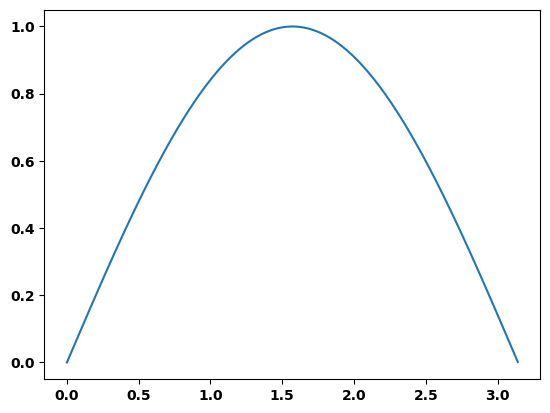
\includegraphics{PresentationOfCommunicatingCode_files/figure-pdf/cell-3-output-1.png}

}

\end{figure}

\hypertarget{but-not-everyone-loves-notebooks}{%
\subsection{But Not everyone loves notebooks
:(}\label{but-not-everyone-loves-notebooks}}

Notebooks have their \emph{validish} detractors
\href{https://www.youtube.com/watch?v=7jiPeIFXb6U}{I don't like
notebooks.- Joel Grus Youtube}

\url{https://www.youtube.com/embed/7jiPeIFXb6U}

\hypertarget{notebooks-opinion}{%
\subsection{Notebooks Opinion}\label{notebooks-opinion}}

Although notebooks have their \emph{validish} detractors
\href{https://www.youtube.com/watch?v=7jiPeIFXb6U}{I don't like
notebooks.- Joel Grus Youtube} I think if you approach them in the right
way they are a super powerful tool.

The negatives seem to be:

\begin{itemize}
\tightlist
\item
  encourage bad practice in code (a genuine problem)
\item
  issues around order of what cell is run (easily got around with good
  practice)
\item
  issues around lack of auto complete (I don't see the issue, use in
  visual studio autocomplete is there)
\item
  no grammar/spelling correction
\item
  issues with using git and version control

  \begin{itemize}
  \tightlist
  \item
    there are ways around this though
  \end{itemize}
\end{itemize}

\hypertarget{notebook-benefits}{%
\subsection{Notebook Benefits}\label{notebook-benefits}}

\begin{itemize}
\tightlist
\item
  Notebooks are \textbf{intuitive}

  \begin{itemize}
  \tightlist
  \item
    You have the code then the result of the code
  \item
    Plus can add details of how code works
  \item
    And it's linear
  \end{itemize}
\item
  Can get things up and working \textbf{quickly}
\item
  Aid with communicating code
\item
  Encourages \textbf{Writing}

  \begin{itemize}
  \tightlist
  \item
    and writing things down aids thinking in the now and understanding
    what you did and why in the future\\
  \item
    \href{https://www.fast.ai/posts/2019-05-13-blogging-advice.html}{FastAI
    guide for better blogs}
  \end{itemize}
\item
  Can use shell commands e.g.~\texttt{!pip\ install\ pandas}
\item
  Can use
  \href{https://ipython.readthedocs.io/en/stable/interactive/magics.html}{magic
  commands} e.g.~\texttt{\%\%time} to time a cell
\item
  Easy to convert code to a pipeline
\end{itemize}

With many companies moving towards Python/R from Excel and a varied
level of skills.

\begin{itemize}
\tightlist
\item
  The first of these is particularly important to aid communicating code
\end{itemize}

\hypertarget{example-useage}{%
\section{Example Useage}\label{example-useage}}

\hypertarget{example-documenting-code}{%
\subsection{Example: Documenting Code}\label{example-documenting-code}}

\begin{itemize}
\item
  \href{https://thomashsimm.github.io/PesticideDocs/UK_areas.html}{Here}
  is my website for my research project on pesticides in UK food.
\item
  This is not the same as documentation for a package but there are
  parallels
\end{itemize}

This does a few things:

\begin{itemize}
\tightlist
\item
  Documents the analysis steps I have taken including the code and
  outputs

  \begin{itemize}
  \tightlist
  \item
    Useful for data transparency, useability of the code if needs
    modifiying/adapting, and why I did XYZ
  \end{itemize}
\item
  Provides a way to present the data

  \begin{itemize}
  \tightlist
  \item
    There is a streamlit app, but sometimes I like to be able to see the
    code
  \end{itemize}
\end{itemize}

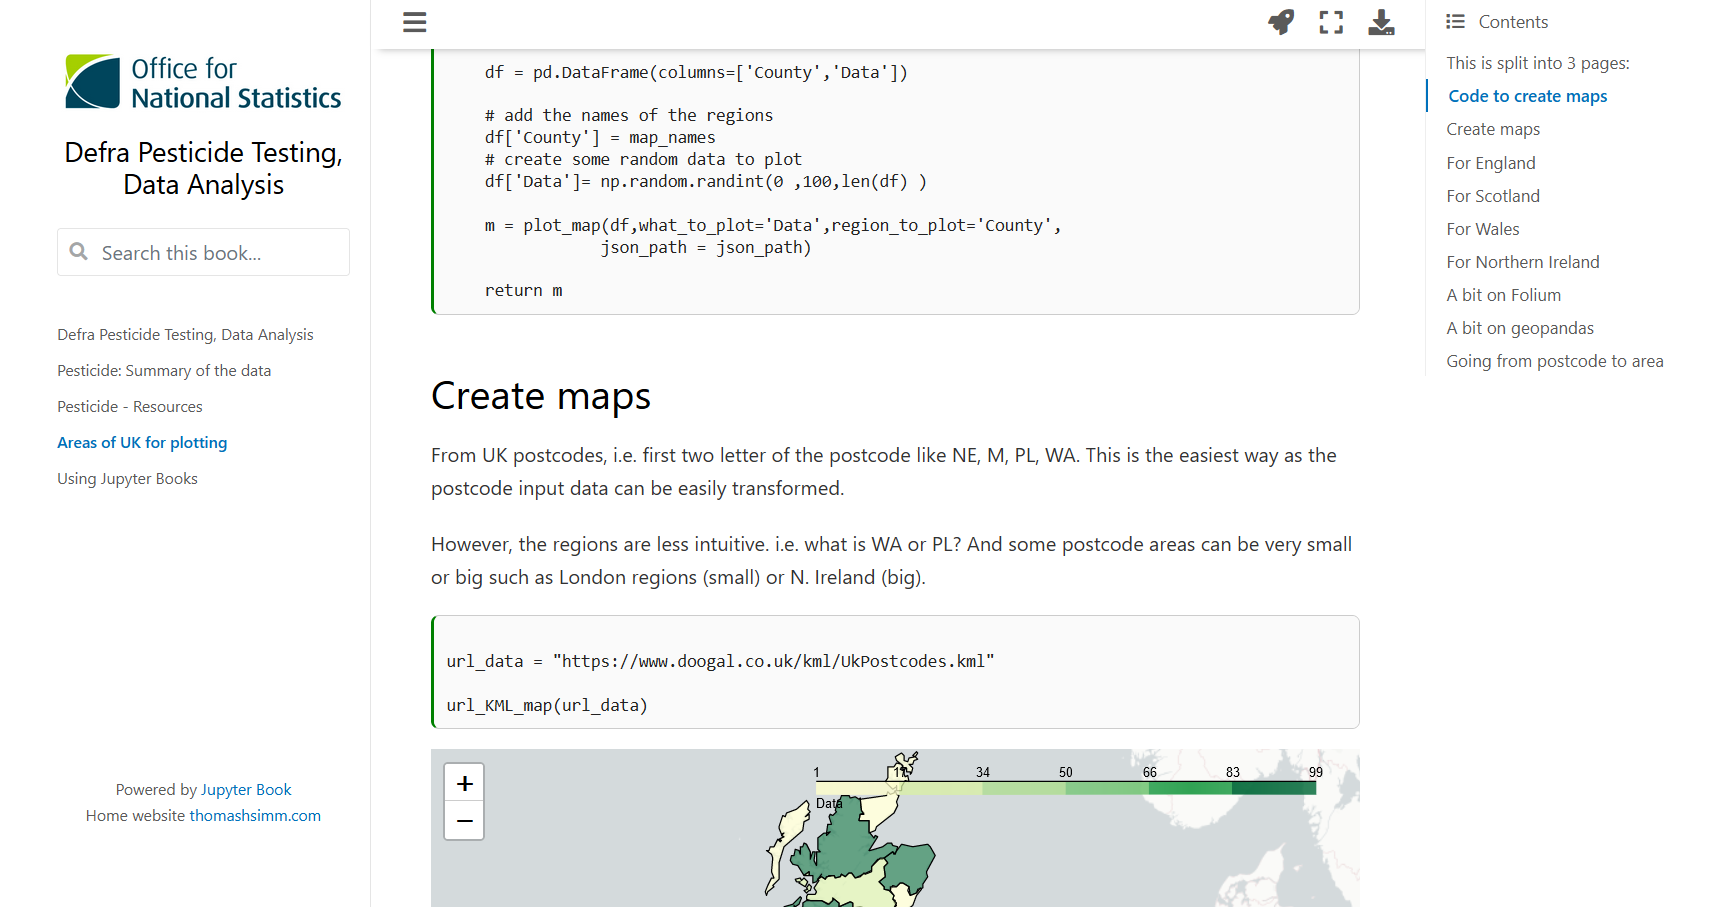
\includegraphics{ghtop_images/pest.png}

\hypertarget{example-tool-to-aid-learning}{%
\subsection{Example: Tool to aid
learning}\label{example-tool-to-aid-learning}}

A big area I have been using Jupyter Notebooks for is to aid learning

\begin{itemize}
\tightlist
\item
  If you want to understand something it helps to write it down
\item
  Having the code next to it is a big advantage
\item
  And if stored on github you can access it anywhere
\end{itemize}

\href{https://thomashsimm.com/tensorflow/2022/09/28/Tensorflow.html}{Tensoflow
cheat sheet} 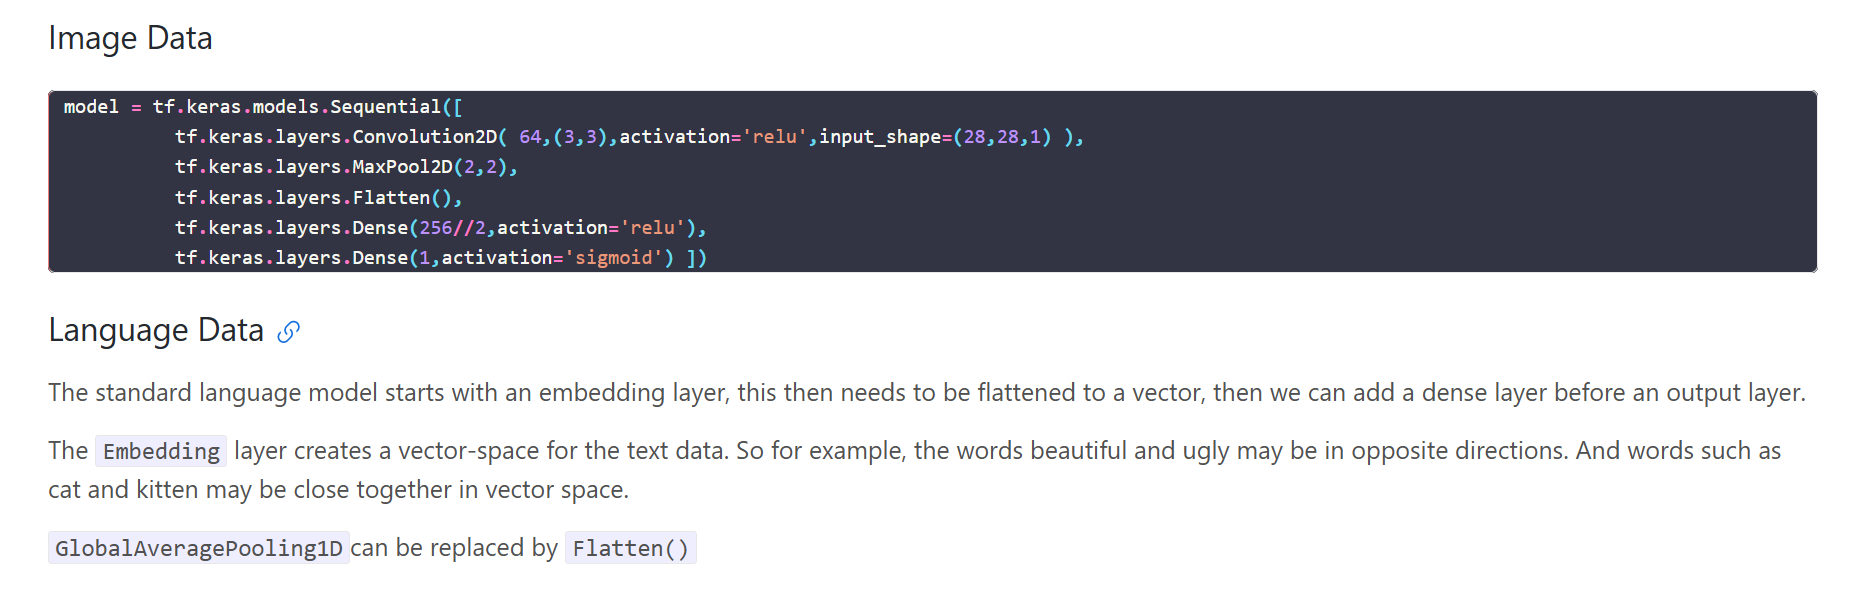
\includegraphics{ghtop_images/tflow.png}

\hypertarget{example-debugging-code}{%
\subsection{Example: Debugging Code}\label{example-debugging-code}}

\begin{itemize}
\tightlist
\item
  Since starting at ONS I have been working with understanding an
  existing project and latterly adding code to it
\item
  The project consists of multiple python files across several folders

  \begin{itemize}
  \tightlist
  \item
    My Python was good but lots of the functions and their useage
    weren't immediately obvious to me
  \end{itemize}
\item
  \textbf{break-points} in VS Studio is really good to step through the
  code and work out what happens in the code.

  \begin{itemize}
  \tightlist
  \item
    I had not used before with Python (but had lots with MATLAB), and
    it's really useful
  \end{itemize}
\item
  But it can be limited what you can do

  \begin{itemize}
  \tightlist
  \item
    difficult to probe code if want to write more than 1 line of code
  \item
    the experience/knowledge exists as you go through it but no
    documentation to refer to later, e.g.~function X does this when I
    give it Y etc
  \end{itemize}
\end{itemize}

\hypertarget{example-debugging-code-2}{%
\subsection{Example: Debugging Code 2}\label{example-debugging-code-2}}

\begin{itemize}
\tightlist
\item
  By copying and pasting code into Jupyter cells I could see and
  document how they worked (e.g.~changing inputs)

  \begin{itemize}
  \tightlist
  \item
    This (copying and pasting) would get around code changes too (which
    would be an issue if modules were just imported)
  \item
    because this was all done in Jupyter notebook I can have a ipynb
    code file and a html file showing how the code works
  \item
    I could even save a pickle file of the variables at a particularly
    point to understand how the code would work from this point
  \end{itemize}
\end{itemize}

\hypertarget{streamlit}{%
\section{Streamlit}\label{streamlit}}

\hypertarget{streamlit-overview}{%
\subsection{Streamlit Overview}\label{streamlit-overview}}

\begin{quote}
Streamlit is an open-source Python library that makes it easy to create
and share beautiful, custom web apps for machine learning and data
science. In just a few minutes you can build and deploy powerful data
apps. So let's get started!
\end{quote}

Principally used to create apps, but some of the functionality works
well for code/data presentations

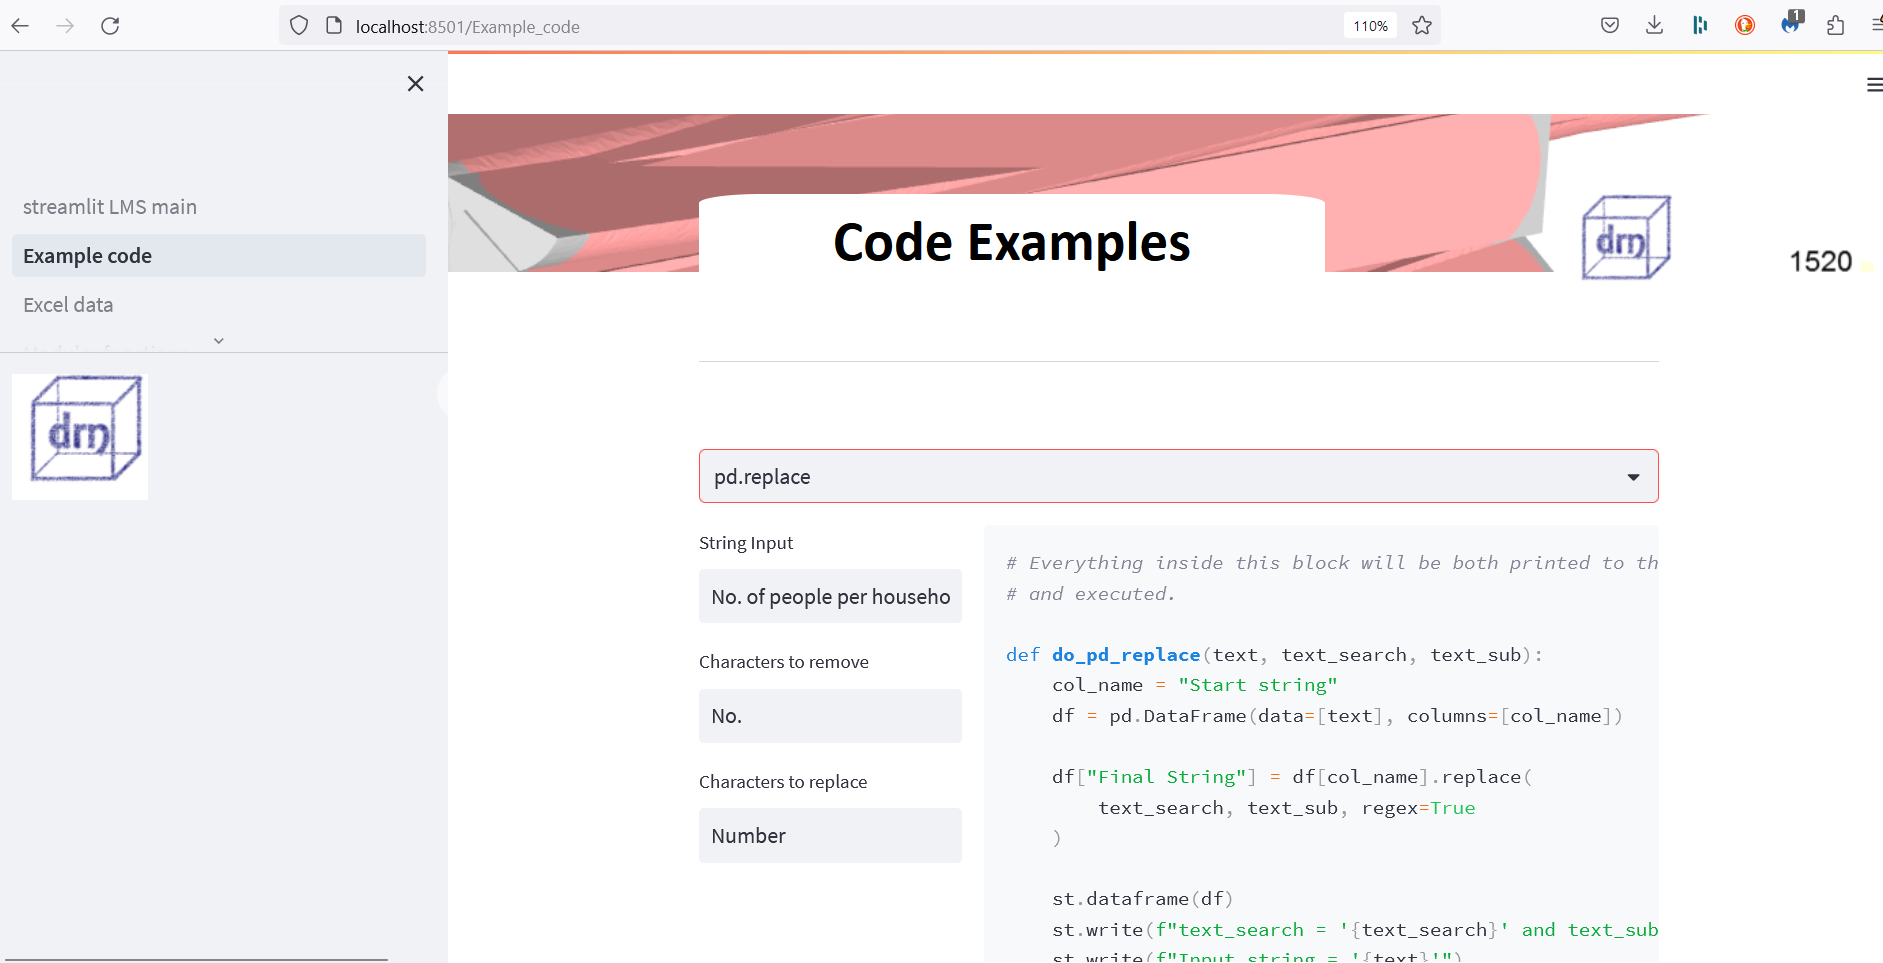
\includegraphics{ghtop_images/streamlit_eg.png}

\hypertarget{streamlit-functionality-overview}{%
\subsection{Streamlit Functionality:
overview}\label{streamlit-functionality-overview}}

Streamlit allows various
\href{https://docs.streamlit.io/library/api-reference}{functionality}:

\begin{itemize}
\tightlist
\item
  textbox
\item
  images/videos
\item
  charts/tables
\item
  menus/buttons
\item
  etc
\end{itemize}

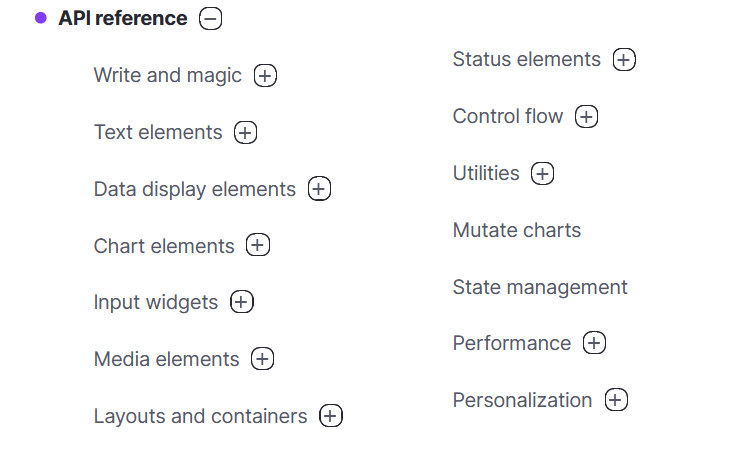
\includegraphics{ghtop_images/streamlit_API.png}

\hypertarget{streamlit-functionality-streamlit_layout}{%
\subsection{Streamlit Functionality:
streamlit\_layout}\label{streamlit-functionality-streamlit_layout}}

But unlike some apps (am thinking MATLAB GUIs) you can't create the look
and functionality separately. So if you want something in a certain
position it can be tricky. HTML can be used with \texttt{st.markdown} to
give more control but it isn't recommended to use by streamlit.

Instead, to create the layout as you would like they have the following
features:

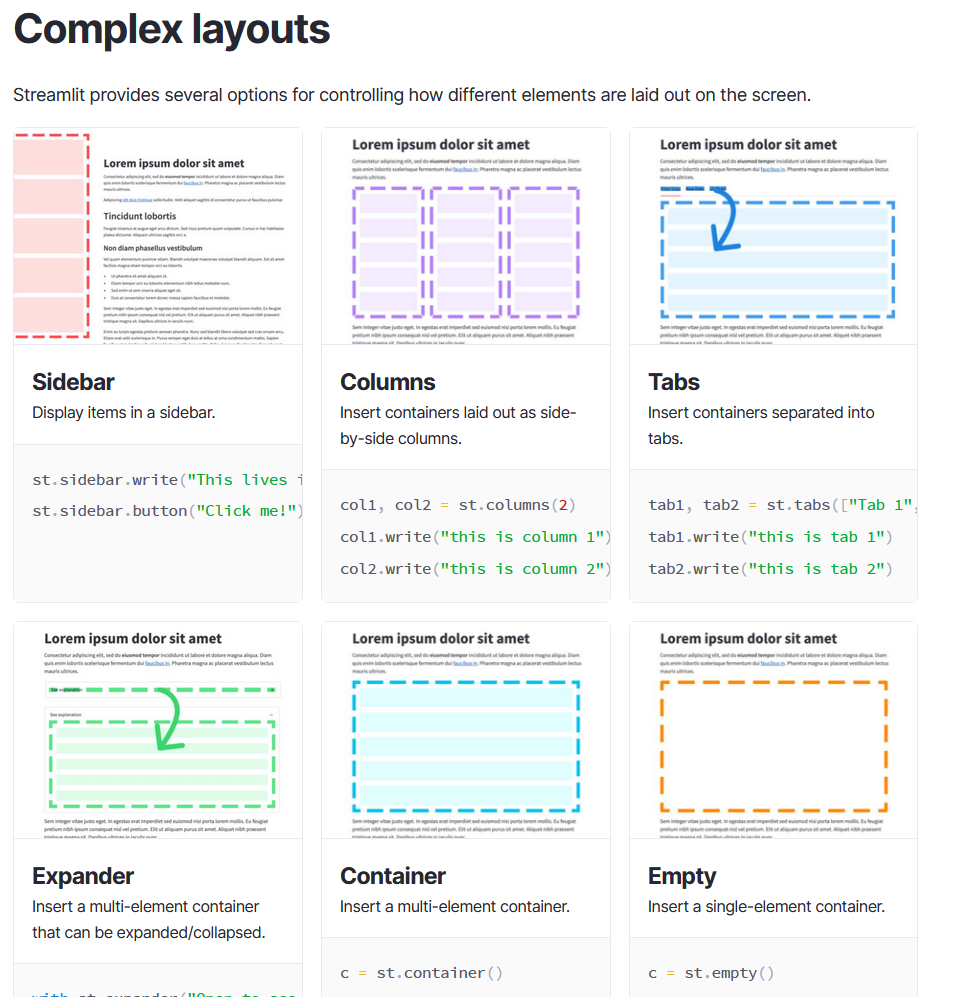
\includegraphics{ghtop_images/streamlit_layout.png}

\hypertarget{streamlit-functionality-columns-and-sidebar}{%
\subsection{Streamlit Functionality: columns and
sidebar}\label{streamlit-functionality-columns-and-sidebar}}

The most useable are the first two: columns and sidebar

Columns allows us to split the app vertically. The code is fairly
simple:

Either \texttt{colL,\ colM,\ colR\ =\ st.columns(3)} for 3 equal columns
or to split columns with different sizes:

\begin{verbatim}
colL, _, colR = st.columns((10, 5, 20))
with colL:
    st.write('On the left')
with colR:
    st.write('On the right twice as big as left')
\end{verbatim}

\texttt{st.sidebar} just adds a sidebar to the app that can be hidden or
shown.

Anything in the sidebar is just prefixed by \texttt{st.sidebar} so:

\begin{verbatim}
st.sidebar.write('I am in the sidebar')
st.write('I am in the main app')
st.sidebar.write('I am back in the sidebar')
\end{verbatim}

\hypertarget{streamlit-functionality-html}{%
\subsection{Streamlit Functionality:
html}\label{streamlit-functionality-html}}

It is possible to add various additional personalisations using html.
BUT it does come with security risks and so is {[}not
recommended{]}{]}(https://github.com/streamlit/streamlit/issues/152)

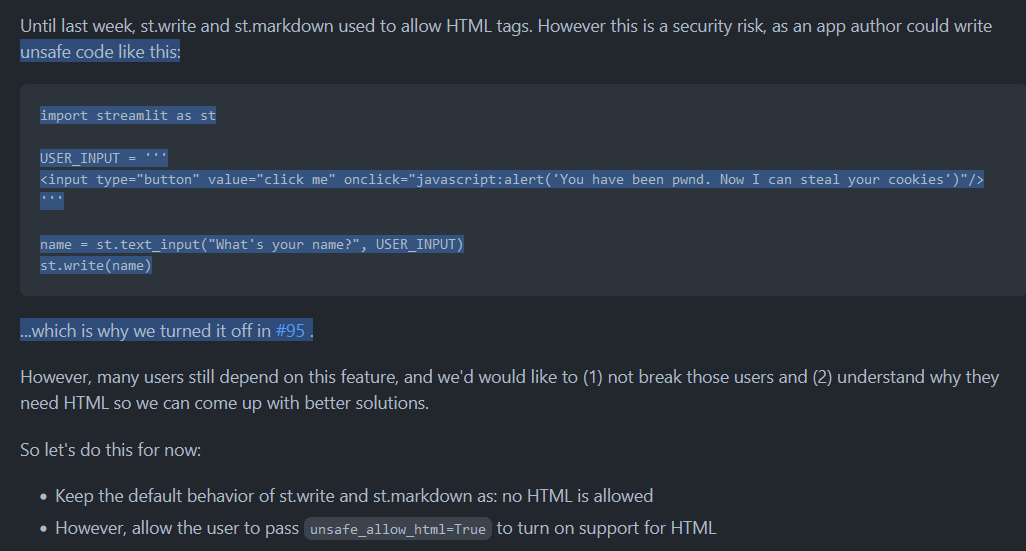
\includegraphics{ghtop_images/streamlit_html.png}

But it does allow much more control over the layout of the app that can
be useful for a presentation: - Can add a background image - Can add
background color to a textbox - Control over positioning of widgets -
lots more

HTML is implementated using \texttt{st.markdown} with
\texttt{unsafe\_allow\_html=True} inside the former

\hypertarget{streamlit-functionality-html-examples}{%
\subsection{Streamlit Functionality: html
examples}\label{streamlit-functionality-html-examples}}

add background to a text box

\begin{verbatim}
text = "Code Examples"
        st.markdown(f'<center><p style=font-family:"Calibri";background-color:#FFFFFF;color:#000000;font-size:42px;border-radius:10%><b>{text}</b></p></center>', unsafe_allow_html=True)
\end{verbatim}

Or to add a background image

\begin{verbatim}
import streamlit as st
import base64

@st.cache(allow_output_mutation=True)
def get_base64_of_bin_file(bin_file):
    with open(bin_file, 'rb') as f:
        data = f.read()
    return base64.b64encode(data).decode()

def set_png_as_page_bg(png_file):
    bin_str = get_base64_of_bin_file(png_file) 
    page_bg_img = '''
    <style>
    .stApp {
    background-image: url("data:image/png;base64,%s");
    background-size: contain;
    background-repeat: no-repeat;
    background-attachment: scroll; # doesn't work
    }
    </style>
    ''' % bin_str
    st.markdown(page_bg_img, unsafe_allow_html=True)
    return
\end{verbatim}

\hypertarget{streamlit-functionality-echo}{%
\subsection{Streamlit Functionality:
echo}\label{streamlit-functionality-echo}}

\begin{quote}
Sometimes you want your Streamlit app to contain both your usual
Streamlit graphic elements and the code that generated those elements.
That's where st.echo() comes in
\end{quote}

Easier to display this by an example:

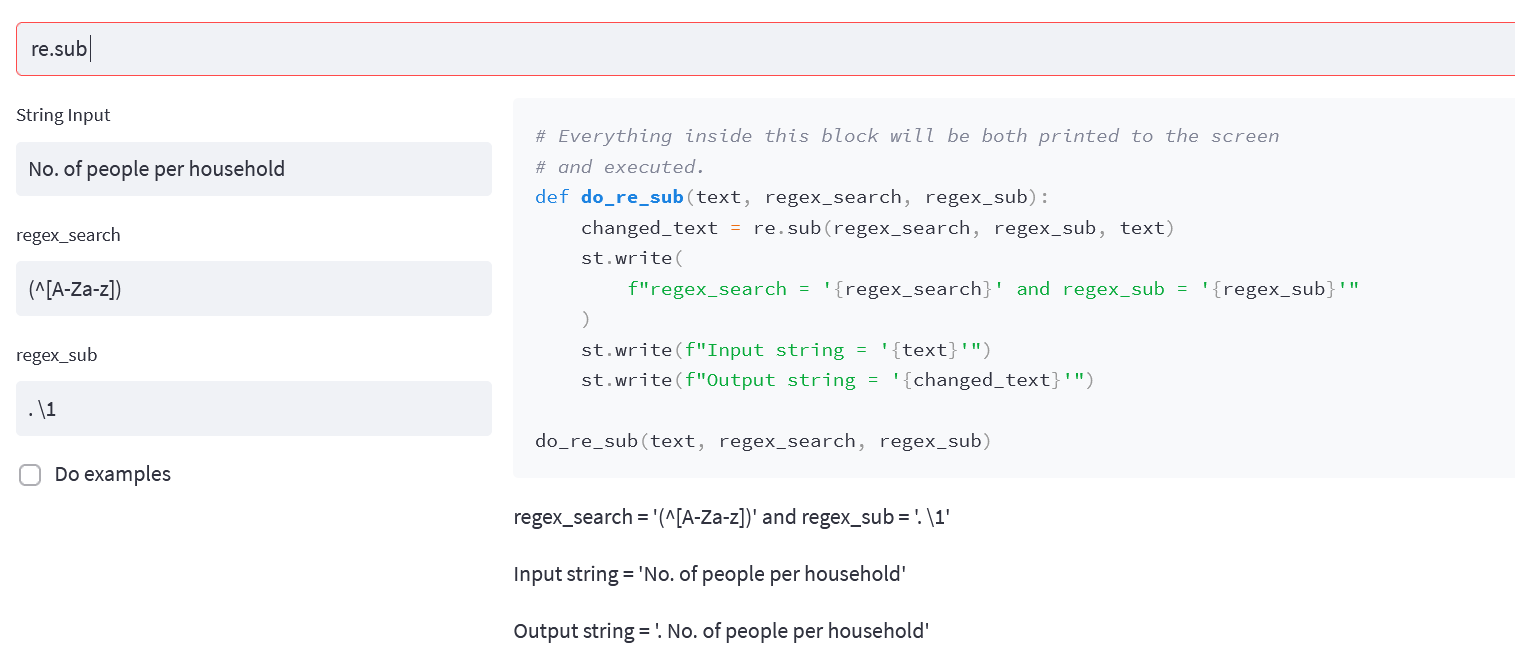
\includegraphics{ghtop_images/streamlit_echo.png}

In the example above the right of the image is given below (st.columns
is used, where the input for the function is found from the left
column).

\begin{itemize}
\tightlist
\item
  \texttt{st.echo} is used with the \texttt{with} statement.
\item
  everything within the \texttt{with} is printed to the screen and
  executed
\end{itemize}

\begin{verbatim}
with st.echo():
    # Everything inside this block will be both printed to the screen
    # and executed.

    def do_pd_replace(text, text_search, text_sub):
        col_name = "Start string"
        df = pd.DataFrame(data=[text], columns=[col_name])

        df["Final String"] = df[col_name].replace(
            text_search, text_sub, regex=True
        )

        st.dataframe(df)
        st.write(f"text_search = '{text_search}' and text_sub = '{text_sub}'")
        st.write(f"Input string = '{text}'")
        st.write(f"Output string = '{df['Final String'].values[0]}'")

    do_pd_replace(text, text_search, text_sub)
\end{verbatim}

\hypertarget{streamlit-functionality-pages}{%
\subsection{Streamlit Functionality:
pages}\label{streamlit-functionality-pages}}

By simply creating a folder called \texttt{pages} and putting other
streamlit .py files in the folder they can then be accessed in the
sidebar.

\begin{itemize}
\tightlist
\item
  A main file needs to be outside the pages folder
\item
  The .py files in pages behave as if they were outside the folder
  (i.e.~when loading files/functions)
\end{itemize}

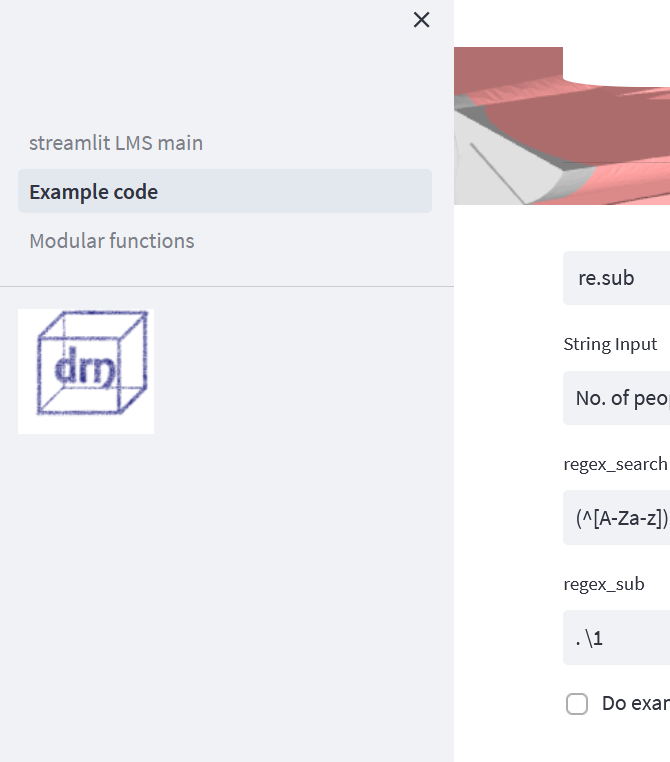
\includegraphics{ghtop_images/streamlit_pages.png}

\hypertarget{example-streamlit-presentation}{%
\subsection{Example Streamlit
Presentation}\label{example-streamlit-presentation}}

\includegraphics{ghtop_images/streamlit_present.webm}

\hypertarget{notebooks-to-html}{%
\section{Notebooks to HTML}\label{notebooks-to-html}}

\hypertarget{what-i-have-used-to-convert-notebooks-to-html}{%
\subsection{What I have used to convert notebooks to
html}\label{what-i-have-used-to-convert-notebooks-to-html}}

\begin{itemize}
\tightlist
\item
  \href{https://fastpages.fast.ai/}{fastpages}

  \begin{itemize}
  \tightlist
  \item
    Previously I converted notebooks to html via fastpages but this is
    now deprecated and they are recommending the use of quarto.
  \end{itemize}
\item
  \href{https://quarto.org/}{quarto}

  \begin{itemize}
  \tightlist
  \item
    So far I have found \textbf{quarto} really good and flexible
    (\emph{N.B. R works too})
  \item
    Easy to convert a notebook to multiple formats, including html,
    powerpoint, pdf, word doc
  \item
    \textbf{BUT} Quarto is not possible if installing from non pip
    sources is an issue (as far as I can tell currently)
  \end{itemize}
\item
  \href{https://nbconvert.readthedocs.io/en/latest/}{nbconvert} is
  another option I tried

  \begin{itemize}
  \tightlist
  \item
    but it doesn't seem to have the functionality of fastpages or
    quarto.
  \end{itemize}
\item
  \href{https://jupyterbook.org/en/stable/intro.html}{Jupyter Books}
  seems to be the best option within companies with installation issues

  \begin{itemize}
  \tightlist
  \item
    Maybe not as good as quarto but it works!
  \end{itemize}
\end{itemize}

\hypertarget{others}{%
\subsection{Others}\label{others}}

\begin{itemize}
\tightlist
\item
  I know some people use
  \href{https://www.sphinx-doc.org/en/master/}{Sphinx},

  \begin{itemize}
  \tightlist
  \item
    is recommended by QA
  \item
    From what
    \href{https://www.sphinx-doc.org/en/master/tutorial/index.html}{I
    can tell sphinx} on it's own is not as easy to use as notebooks
  \item
    But there is a jupyter extension
    \href{https://nbsphinx.readthedocs.io/en/0.8.10/}{nbsphinx}
  \item
    Jupyter Books uses Sphinx heavily
    \href{https://jupyterbook.org/en/stable/explain/sphinx.html}{under
    the hood}
  \end{itemize}
\item
  \href{https://nbdev.fast.ai/getting_started.html}{nbdev}

  \begin{itemize}
  \tightlist
  \item
    I think is connected to quarto
  \end{itemize}
\item
  \href{https://github.com/voila-dashboards/voila}{Voila}

  \begin{itemize}
  \tightlist
  \item
    Voilà turns Jupyter notebooks into standalone web applications.
  \item
    Looks good, bit like streamlit
  \item
    but seems to interfere with other libraries
  \item
    \href{https://github.com/mljar/mercury}{mercury} seems similar
  \end{itemize}
\end{itemize}

\hypertarget{creating-html-other-formats}{%
\subsection{Creating html (\& other
formats)}\label{creating-html-other-formats}}

\hypertarget{quarto}{%
\subsubsection{\texorpdfstring{\href{https://quarto.org/docs/get-started/hello/vscode.html}{Quarto}}{Quarto}}\label{quarto}}

Installation is via a package i.e.~\texttt{.msi} for Windows or
\texttt{.pkg} for Mac. Which can cause issues.

Works with both \texttt{ipynb} and \texttt{qmd} files, which are both a
mixture of markdown and executable code.

The only thing that needs to be done with the notebook is add a YAML
block at the start of the notebook, like the following (raq not markdown
was used):

\begin{verbatim}
---
title: "Communicating code: Website"
subtitle: "Using the notebook format for a website"
author: "Thomas H. Simm"
format:
  html:
    toc: true
title-slide-attributes:
  data-background-size: contain
  data-background-opacity: "0.5"
jupyter: python3
---
\end{verbatim}

We can create different files from this .ipynb Jupyter notebook using
the following code:

\begin{itemize}
\tightlist
\item
  \texttt{quarto\ render\ testPres.ipynb\ -\/-to\ pptx}
\item
  \texttt{quarto\ render\ testPres.ipynb\ -\/-to\ pdf}
\item
  \texttt{quarto\ render\ testPres.ipynb\ -\/-to\ html}
\item
  \texttt{quarto\ render\ testPres.ipynb\ -\/-to\ revealjs}
\end{itemize}

Further, formatting for projects (i.e.~for website) can be done within
the
\href{https://quarto.org/docs/projects/quarto-projects.html\#shared-metadata}{configuration
file} \texttt{\_quarto.yml}

\begin{verbatim}
project:
  type: website
  output-dir: _site

website:
  title: "ThomasHSimm"
  favicon: /posts/Picture3.png
  body-header: <img src="/posts/header2.png" height=200>

  navbar:
    right:
      - about.qmd
      - icon: github
        href: https://github.com/ThomasHSimm
      - icon: mortarboard-fill
        href: https://scholar.google.com/citations?hl=en&user=HdPDn1sAAAAJ
format:
  html:
    theme: 
      light: flatly
      dark: darkly
    css: styles.css
\end{verbatim}

\hypertarget{jupyter-books}{%
\subsection{\texorpdfstring{\href{https://jupyterbook.org/en/stable/basics/build.html}{Jupyter
Books}}{Jupyter Books}}\label{jupyter-books}}

We can create different files from this .ipynb Jupyter notebook using
the following code:

\begin{itemize}
\tightlist
\item
  \texttt{jupyter-book\ build\ .\textbackslash{}PesticideDocs\textbackslash{}}
\item
  \texttt{jupyter-book\ build\ \textless{}path-to-book\textgreater{}}
\item
  \texttt{jupyter-book\ build\ \textless{}path-to-book\textgreater{}\ -\/-builder\ pdfhtml}
\item
  \texttt{jupyter-book\ build\ \textless{}path-to-book\textgreater{}\ -\/-builder\ singlehtml}
\end{itemize}

The only difference in notebook is that it needs to have One header in a
markdown cell for the table of contents, e.g.~

\texttt{\#\ Title\ of\ page}

\hypertarget{configuration-file}{%
\subsection{Configuration file}\label{configuration-file}}

A seperate files \texttt{\_config.yml} is used to define how the html
(or other) files will look

\begin{verbatim}
# Book settings
# Learn more at https://jupyterbook.org/customize/config.html

title: Defra Pesticide Testing, Data Analysis
author: Thomas Simm
logo: ONS-logo.png
exclude_patterns: [_build, Thumbs.db, .DS_Store, "**.ipynb_checkpoints"]


# Force re-execution of notebooks on each build.
# See https://jupyterbook.org/content/execute.html
execute:
  execute_notebooks: force

# Define the name of the latex output file for PDF builds
latex:
  latex_documents:
    targetname: book.tex

# Add a bibtex file so that we can create citations
bibtex_bibfiles:
  - references.bib

# Information about where the book exists on the web
repository:
  url: https://github.com/ThomasHSimm/Pesticide  # Online location of your book
  path_to_book: docs  # Optional path to your book, relative to the repository root
  branch: master  # Which branch of the repository should be used when creating links (optional)

# Add GitHub buttons to your book
# See https://jupyterbook.org/customize/config.html#add-a-link-to-your-repository
# HTML-specific settings
html:
  favicon                   : "_images/favicon.jpg"  # A path to a favicon image
  use_edit_page_button      : false  # Whether to add an "edit this page" button to pages. If `true`, repository information in repository: must be filled in
  use_repository_button     : false  # Whether to add a link to your repository button
  use_issues_button         : false  # Whether to add an "open an issue" button
  use_multitoc_numbering    : true   # Continuous numbering across parts/chapters
  extra_navbar              : Powered by <a href="https://jupyterbook.org">Jupyter Book</a>
                              <br>Home website <a href="https://thomashsimm.com/">thomashsimm.com</a> # Will be displayed underneath the left navbar.
  extra_footer              : ""  # Will be displayed underneath the footer.
  google_analytics_id       : ""  # A GA id that can be used to track book views.
  home_page_in_navbar       : true  # Whether to include your home page in the left Navigation Bar
  baseurl                   : ""  # The base URL where your book will be hosted. Used for creating image previews and social links. e.g.: https://mypage.com/mybook/
  comments:
    hypothesis              : false
    utterances              : false
  announcement              : "" # A banner announcement at the top of the site.
\end{verbatim}

\hypertarget{table-of-content}{%
\subsection{Table of content}\label{table-of-content}}

And in addition to the config file a table of contents file is required
\texttt{\_toc.yml}:

\begin{verbatim}
# Table of contents
# Learn more at https://jupyterbook.org/customize/toc.html

format: jb-book
root: intro
chapters:
- file: Pesticide_Plots
- file: References
- file: UK_areas
- file: using_jupyter_books
\end{verbatim}

\hypertarget{creating-a-webpage-from-this}{%
\subsection{Creating a webpage from
this}\label{creating-a-webpage-from-this}}

Takes about 30 mins including installing the chosen converter.
\emph{(But can be done much quicker)}

\begin{itemize}
\tightlist
\item
  create a Github repo for your website
\item
  choose the converter (e.g.~Jupyter Books)

  \begin{itemize}
  \tightlist
  \item
    And follow their instructions
  \end{itemize}
\item
  go to settings -\textgreater{} Pages within the repo

  \begin{itemize}
  \tightlist
  \item
    few options to do
  \end{itemize}
\item
  Optional: add your own website url to it
\end{itemize}

Link how to do this
\href{https://kirenz.github.io/codelabs/codelabs/jupyter-book/\#7}{here}

In Quarto a command from your PC in the repo, publishes the website:

\texttt{quarto\ publish\ quarto-pub}

Or equivalently with
\href{https://jupyterbook.org/en/stable/publish/gh-pages.html}{Jupyter
Books}:

\texttt{ghp-import\ -n\ -p\ -f\ \_build/html}

\hypertarget{creating-directly-from-the-repo}{%
\subsection{Creating directly from the
repo}\label{creating-directly-from-the-repo}}

If we instead want to convert notebook files directly from a repo to
create a website then this can be done with
\href{https://docs.netlify.com/}{Netlify}.

This is useful if using Gitlab (i.e.~not Github) or don't want all the
extra html files cluttering the repo.

\hypertarget{steps}{%
\subsubsection{Steps:}\label{steps}}

\url{https://jupyterbook.org/en/stable/publish/netlify.html}

\begin{itemize}
\tightlist
\item
  Sign up and connect Github/Gitlab
\item
  Add a \texttt{requirements.txt} file and also toc.yml to directory
\item
  On netlify -\textgreater{} Add new site -\textgreater{} import from an
  existing repo
\item
  Insert something like below

  \begin{itemize}
  \tightlist
  \item
    N.B. the command:
  \item
    \texttt{pip\ install\ -r\ requirements.txt\ \&\&\ jupyter-book\ build\ .}
  \item
    and folder location
  \end{itemize}
\end{itemize}

\hypertarget{on-netlify}{%
\subsection{On netlify}\label{on-netlify}}

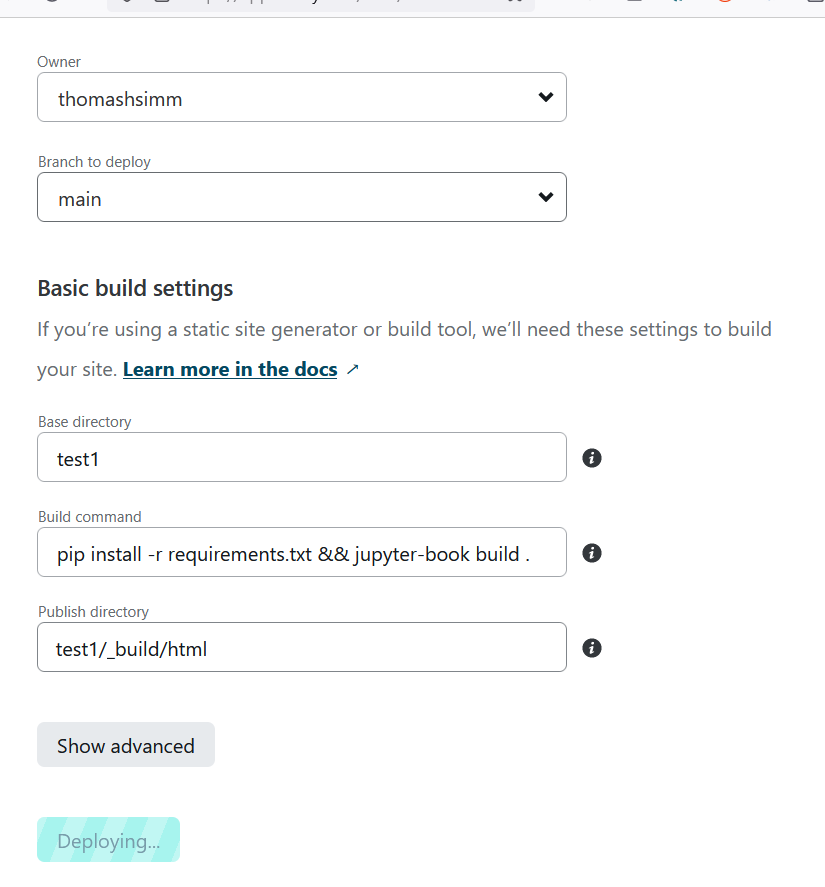
\includegraphics{ghtop_images/netlify.png}

Example:

\begin{itemize}
\tightlist
\item
  \href{https://gitlab.com/ThomasHSimm/test-presentation}{Gitlab repo}
\item
  \href{https://thomashsimm.netlify.app/intro.html}{Resulting website
  https://thomashsimm.netlify.app/intro.html}

  \begin{itemize}
  \tightlist
  \item
    And
    \href{https://63f518d4377f1f00084d90ce--jocular-hotteok-1484e4.netlify.app/intro.html}{from
    the inner folder}
  \end{itemize}
\end{itemize}

\hypertarget{presentations}{%
\section{Presentations}\label{presentations}}

\hypertarget{quarto-presentations}{%
\subsection{Quarto Presentations}\label{quarto-presentations}}

Quarto supports a variety of formats for creating presentations,
including:

\begin{verbatim}
revealjs — reveal.js (HTML)

pptx — PowerPoint (MS Office)

beamer — Beamer (LaTeX/PDF)
\end{verbatim}

I'll consider the first two

\hypertarget{quarto-powerpoint-overview}{%
\subsection{Quarto PowerPoint
overview}\label{quarto-powerpoint-overview}}

The steps to make a PowerPoint presentation from a notebook:

\begin{enumerate}
\def\labelenumi{\arabic{enumi}.}
\tightlist
\item
  Create the inbuilt template.pptx file
\item
  Adjust it to match your own template
\item
  At the top of the notebook insert \texttt{format} for \texttt{pptx}
  including the template file
\item
  Choose how you will define a new page
\item
  You will probably need to manually check the slides and adjust as
  required

  \begin{itemize}
  \tightlist
  \item
    especially for interactive content and code
  \end{itemize}
\end{enumerate}

\hypertarget{creating-the-template}{%
\subsection{Creating the template}\label{creating-the-template}}

\emph{(Office info correct for Office 365 Feb 2023, Version 2301 Build
16.0.16026.20002)}

If your workplace has a custom template or you have one you always use,
you can incorporate this into quarto.

However, quarto is quite specific on the form this template takes, and
requires the following elements - Title Slide - Title and Content -
Section Header - Two Content - Comparison - Content with Caption - Blank

\hypertarget{by-selecting-layout-from-the-home-tab-in-powerpoint-the-different-layouts-can-be-seen}{%
\subsection{By selecting Layout from the Home tab in powerpoint the
different layouts can be
seen}\label{by-selecting-layout-from-the-home-tab-in-powerpoint-the-different-layouts-can-be-seen}}

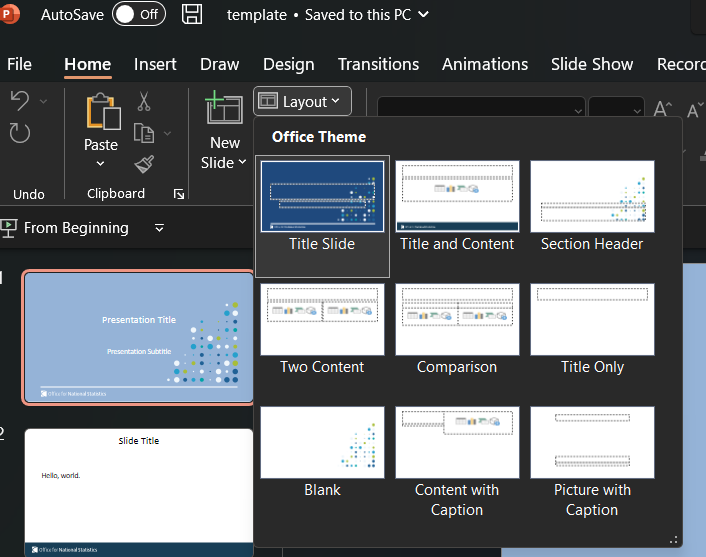
\includegraphics{ghtop_images/ppt_layout.png}

They can then be modified by going to View tab - Slide Master.

If using your own template you will need to match the names of the
slides given above. These can be found by hovering over the slides on
the left or right clicking on one and selecting ``Rename Layout''

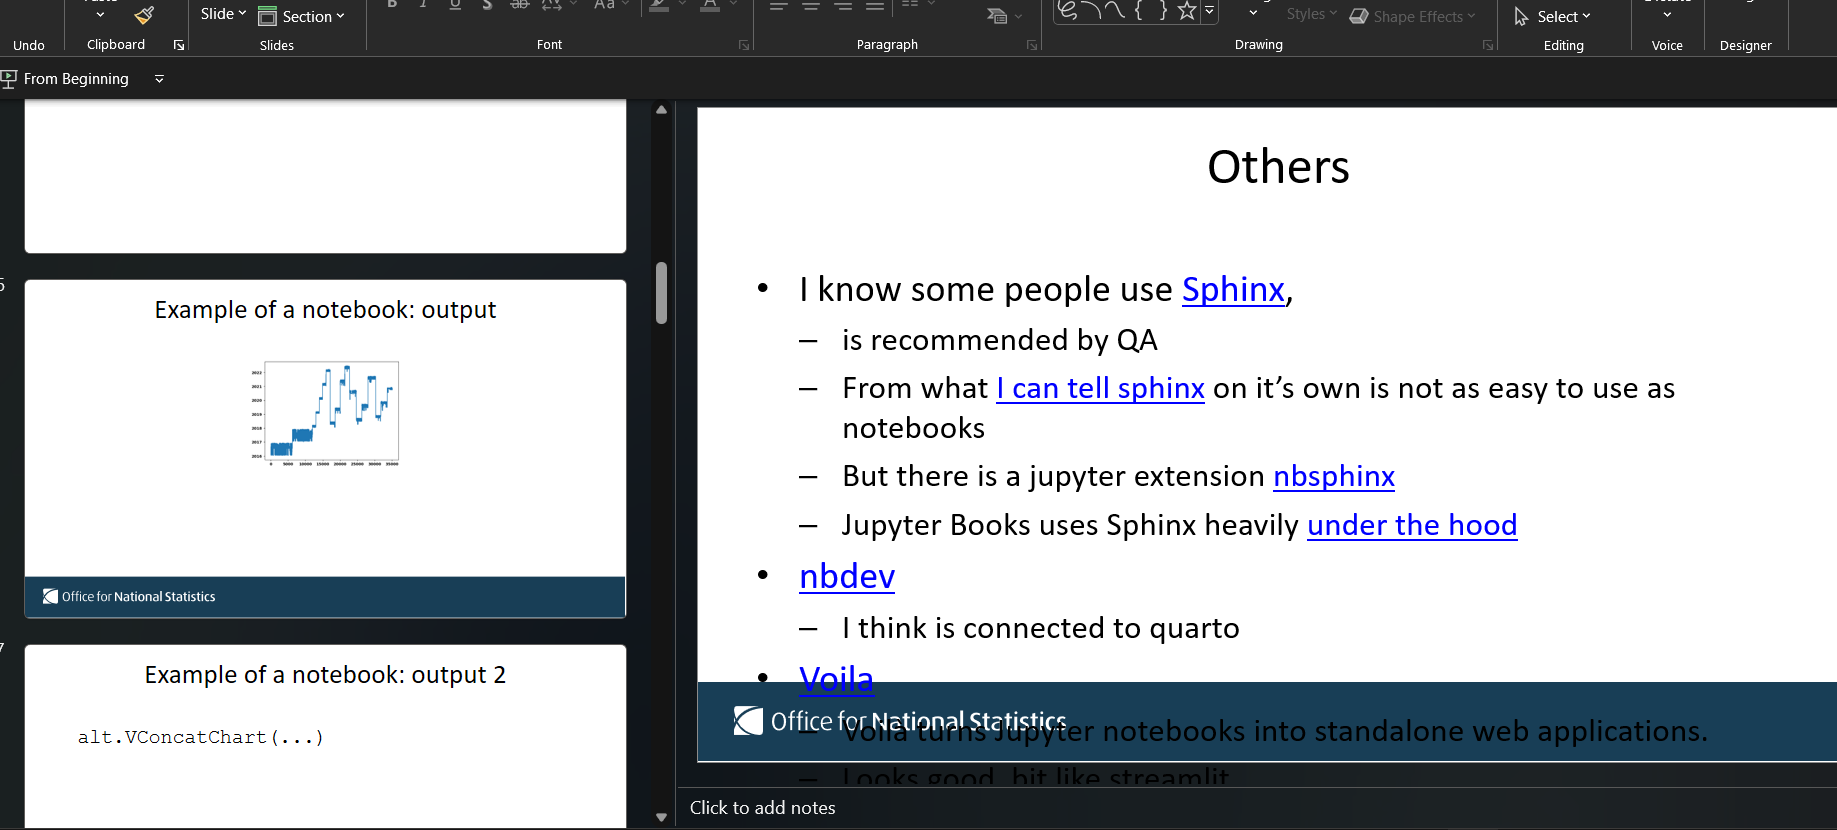
\includegraphics{ghtop_images/ppt_master.png}

Alternatively, create a custom template using quarto and then modify
this. The following command creates the template:

\texttt{quarto\ pandoc\ -o\ template.pptx\ -\/-print-default-data-file\ reference.pptx}

Then go to View tab - Slide Master and modify each slide layout.

Note if you are trying to match a template, some tips: - go to Design
-\textgreater{} Slide Size and match this to your template - when View
tab - Slide Master is selected go to first tab (see above it will be
left indented) on one you are copying from and select all on this then
paste to the new template - these will be background images and other
things that want to be passed to all slides - Check other slides for
images and font-styles etc to match to the new template

\hypertarget{load-the-template}{%
\subsection{Load the template}\label{load-the-template}}

To load the template the first cell in the notebook needs to be modified
as follows to reference the \texttt{template.pptx} file.

\begin{verbatim}
format:
  pptx:
    reference-doc: template.pptx
    slide-level: 2
\end{verbatim}

In addition, we can also specify here the rule by which a new slide is
defined. If \texttt{slide-level:\ 2} is used a new slide is defined by
``\#\#' and a new section header by `\#'. So if we used `\#\#\#' this
would be a heading within the slide.

If \texttt{slide-level:\ 1} is used a new slide is defined by ``\#' and
`\#\#' this would be a heading within the slide (this is normally the
default).

\hypertarget{check-the-slides}{%
\subsection{Check the slides}\label{check-the-slides}}

I have found creation of slides to powerpoint more prone to strange
results than if .doc/.pdf/.html are used.

So check the slides, see if interactive content or code has been
included (probably not) and if the slide content goes outside the slide.

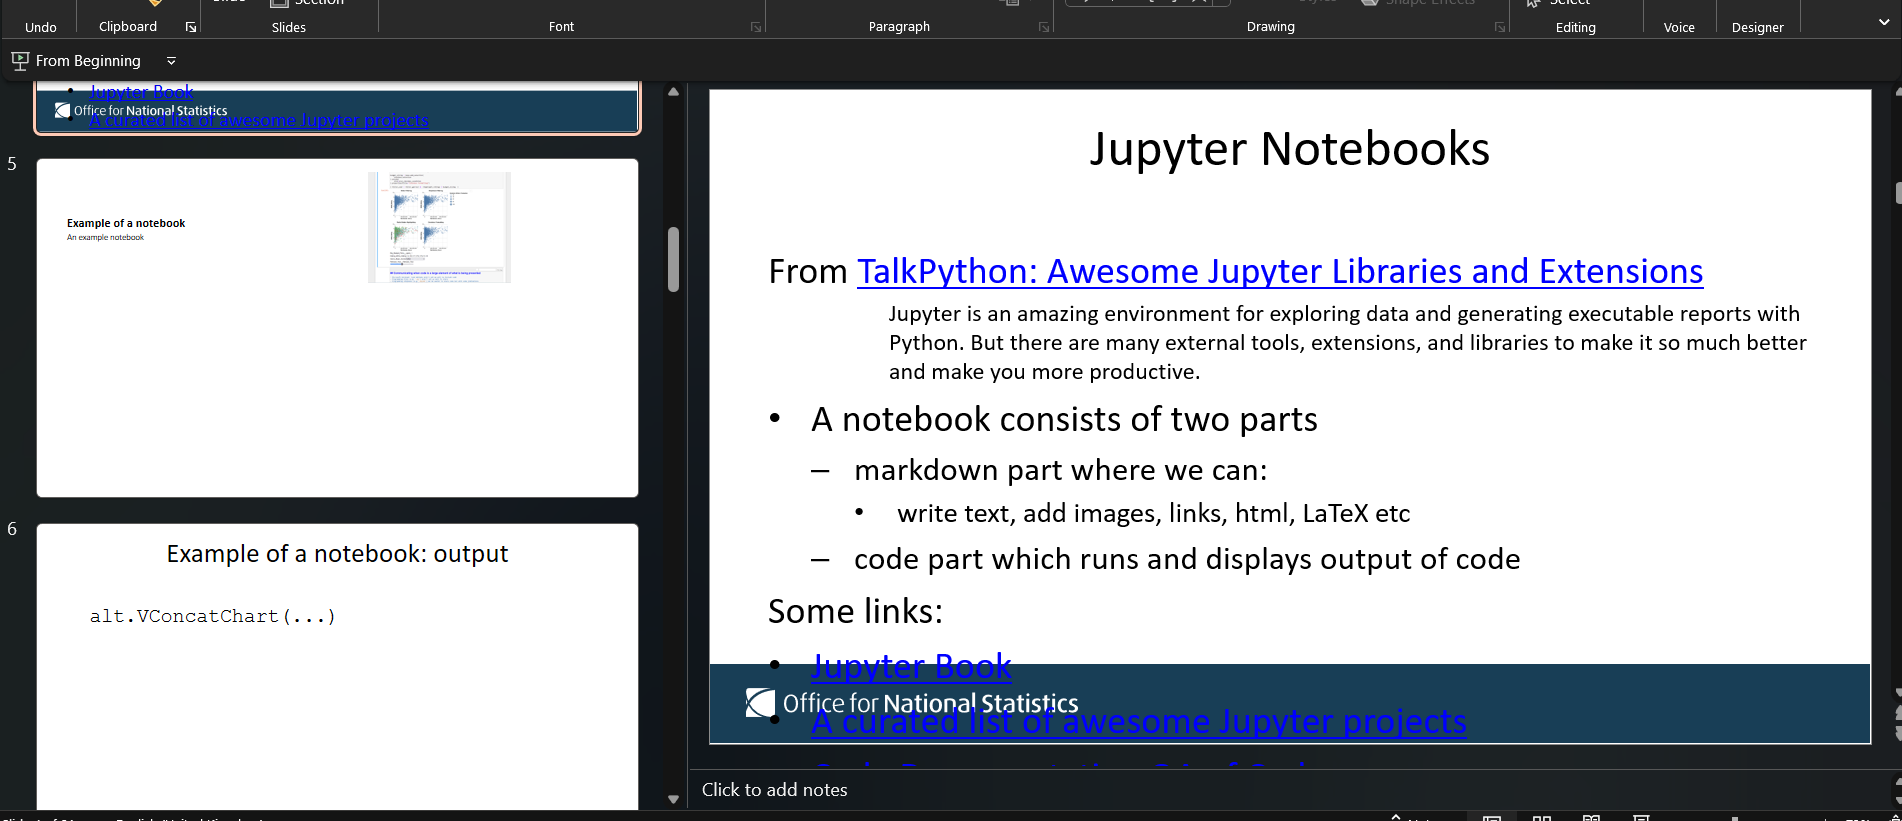
\includegraphics{ghtop_images/ppt_eg.png}

In the example above - There is overlap of text on a slide - Strange
ouput of a slide - Code output not displayed

\hypertarget{quarto-html-overview}{%
\section{Quarto HTML overview}\label{quarto-html-overview}}

With quarto two different html formats can be produced by using either
\texttt{html} or \texttt{revealjs}.

Whereas, \texttt{html} produces the standard html format
\texttt{revealjs} produces an interactive presentation format.
\url{https://quarto.org/docs/presentations/revealjs/}

\texttt{revealjs} does pretty much the same as a powerpoint file but is
more robust - interactive content is included - less issues with getting
format to fit within the slide

But - Can't use the ppt template - And maybe(?) there are issues with
sharing this format? - Interactive elements not as well implemeneted as
within \emph{pure} html

\hypertarget{adding-style-to-revealjs}{%
\subsection{Adding style to revealjs}\label{adding-style-to-revealjs}}

A simple way to add template like details to a \texttt{revealjs} file is
to add a style.css sheet.

In the example below, the style sheet adds logo.png to the bottom right
of each sheet

The file \texttt{style.css} looks like this:

\begin{verbatim}
.reveal .slide-logo {
  display: block;
  position: fixed;
  top: unset !important;
  left: unset !important;
  bottom: 50px;
  right: 12px;
  height: 100px !important;
  width: 100x !important;
  max-width: unset !important;
  max-height: unset !important;
}
\end{verbatim}

And the \texttt{revealjs} part at the top of the jupyter notebook looks
like this

\begin{verbatim}
revealjs:
    slide-number: true
    height: 1080
    width: 1920
    logo: logo.png
    css: style.css
\end{verbatim}

So this would then look like the following, with the logo
(\texttt{logo.png}) in the bottom right, and size and positioning given
by the css file

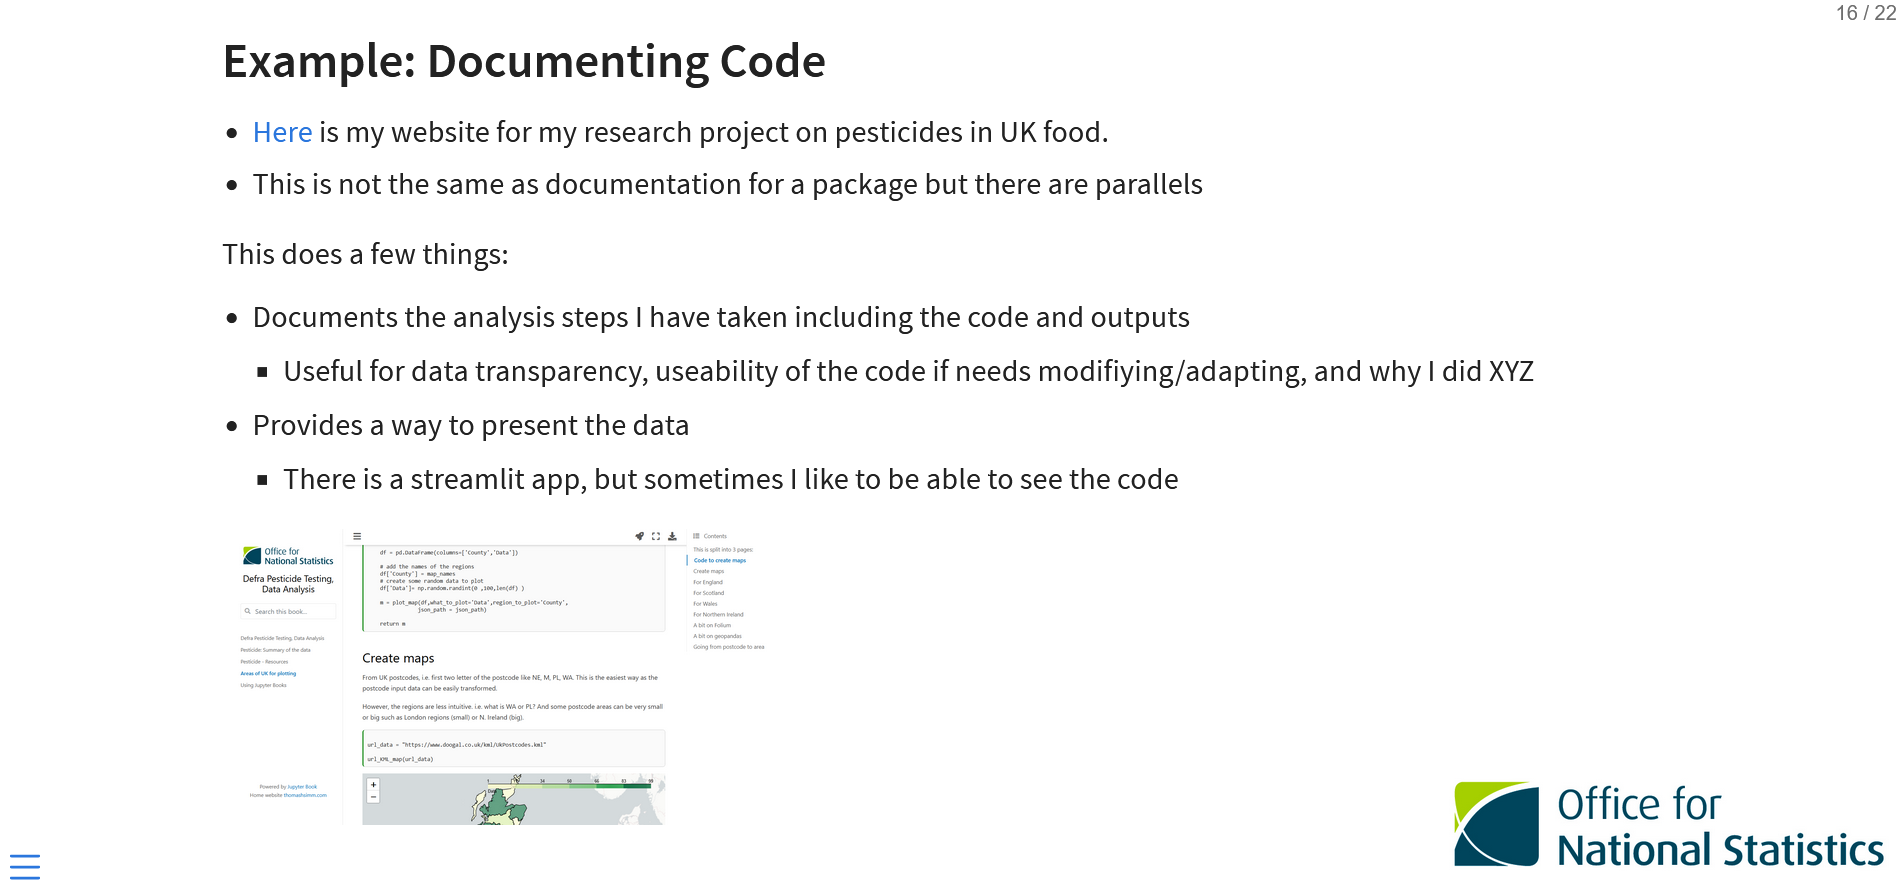
\includegraphics{ghtop_images/ppt_revealstyle.png}

\hypertarget{what-the-revealjs-file-looks-like}{%
\subsection{What the revealjs file looks
like}\label{what-the-revealjs-file-looks-like}}

\includegraphics{ghtop_images/revealjs.mp4}

\hypertarget{tabular-data}{%
\section{Tabular Data}\label{tabular-data}}

\begin{itemize}
\tightlist
\item
  How efficient is Excel when we are just viewing the data?
\item
  What other \emph{with code} options to Excel are there?
\end{itemize}

\hypertarget{excel-files}{%
\subsection{Excel files}\label{excel-files}}

\begin{quote}
\href{https://chat.openai.com/chat}{ChatGPT}: What are the problems of
Excel and xlsx files?
\end{quote}

\begin{enumerate}
\def\labelenumi{\arabic{enumi}.}
\item
  Limited scalability: Excel has a limit on the number of rows and
  columns it can handle effectively.
\item
  Inaccurate data: The manual nature of data entry in Excel can lead to
  errors and inaccuracies.
\item
  Fragility: Complex Excel spreadsheets can break easily if any formula
  or cell reference is altered.
\item
  Lack of security: Excel files are vulnerable to unauthorized access
  and malicious attacks.
\item
  Slow performance: Large and complex Excel files can become slow to
  open and use, leading to decreased productivity.
\item
  Compatibility issues: XLSX files may not be compatible with older
  versions of Excel, or with other software applications.
\item
  Limited collaboration: Sharing Excel files and making changes to them
  can be difficult, especially when multiple people are involved.
\end{enumerate}

For me it is the \textbf{Slow performance} alongside: (a) we are doing
the data manipulation outside Excel anyway and (b) having to have
another application open

\hypertarget{ods-with-excel}{%
\subsubsection{\texorpdfstring{\texttt{ods} with
Excel}{ods with Excel}}\label{ods-with-excel}}

About 10 s to open 3 \texttt{ods} files with Excel

\hypertarget{ods-converted-to-html-in-firefox-browser}{%
\subsubsection{\texorpdfstring{\texttt{.ods} converted to html in
firefox
browser}{.ods converted to html in firefox browser}}\label{ods-converted-to-html-in-firefox-browser}}

About 6 s to open 3 converted \texttt{ods} files in a browser

\hypertarget{ods-converted-to-html-firefox-browser-no-new-tabs}{%
\subsubsection{\texorpdfstring{\texttt{.ods} converted to html firefox
browser no new
tabs}{.ods converted to html firefox browser no new tabs}}\label{ods-converted-to-html-firefox-browser-no-new-tabs}}

Almost instant when open converted \texttt{ods} files in same browser

\hypertarget{what-aspect-of-tables-i-am-considering}{%
\subsection{What aspect of tables I am
considering}\label{what-aspect-of-tables-i-am-considering}}

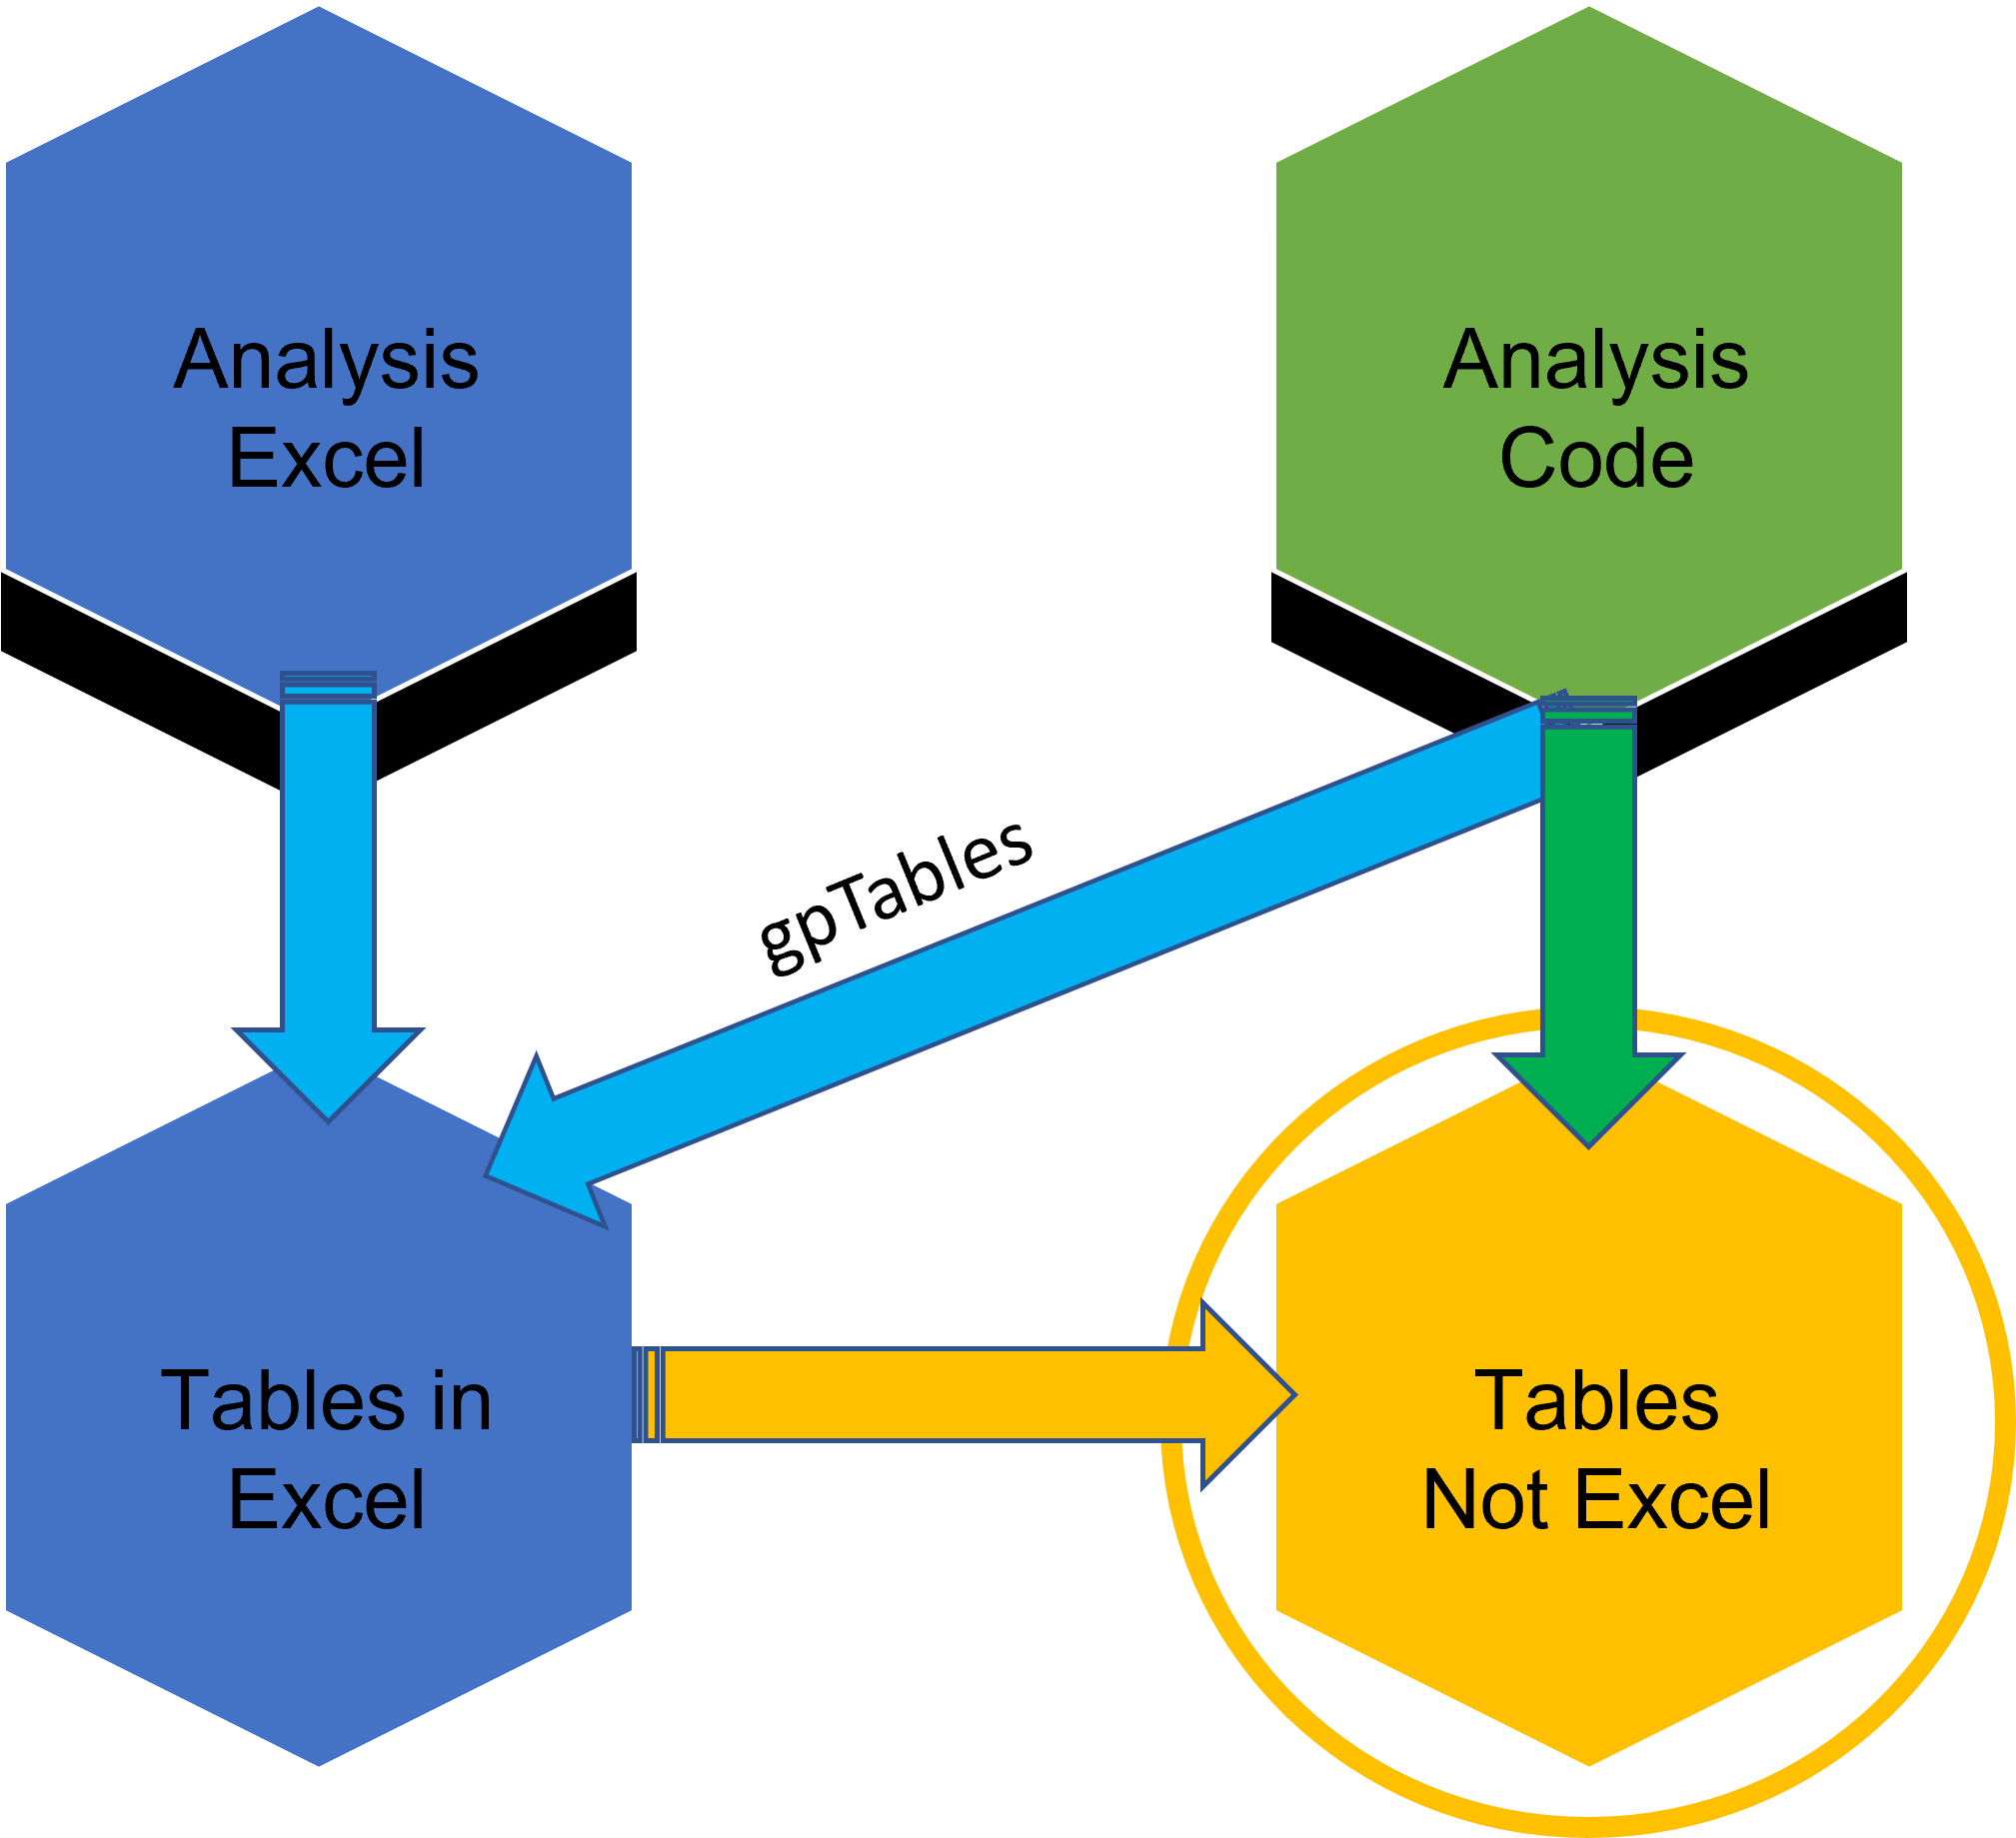
\includegraphics{ghtop_images/tables.png}

\hypertarget{convert-xlsx-to-html}{%
\subsection{Convert xlsx to html?}\label{convert-xlsx-to-html}}

\begin{itemize}
\tightlist
\item
  Opening xlsx files in Excel is slow
\item
  Converting to html if we don't want to edit could be an option
\item
  If we are moving to Python/R aren't non-Excel options worth
  considering??
\end{itemize}

Converting xlsx files to html

\begin{itemize}
\tightlist
\item
  Seems the most obvious course
\item
  But it doesn't seem that easy with code

  \begin{itemize}
  \tightlist
  \item
    but easy within Excel
  \end{itemize}
\end{itemize}

\hypertarget{what-does-chatgpt-say-to-convert-excel-file}{%
\subsection{What does chatgpt say to convert excel
file?}\label{what-does-chatgpt-say-to-convert-excel-file}}

\begin{quote}
Convert an excel file to html with python
\end{quote}

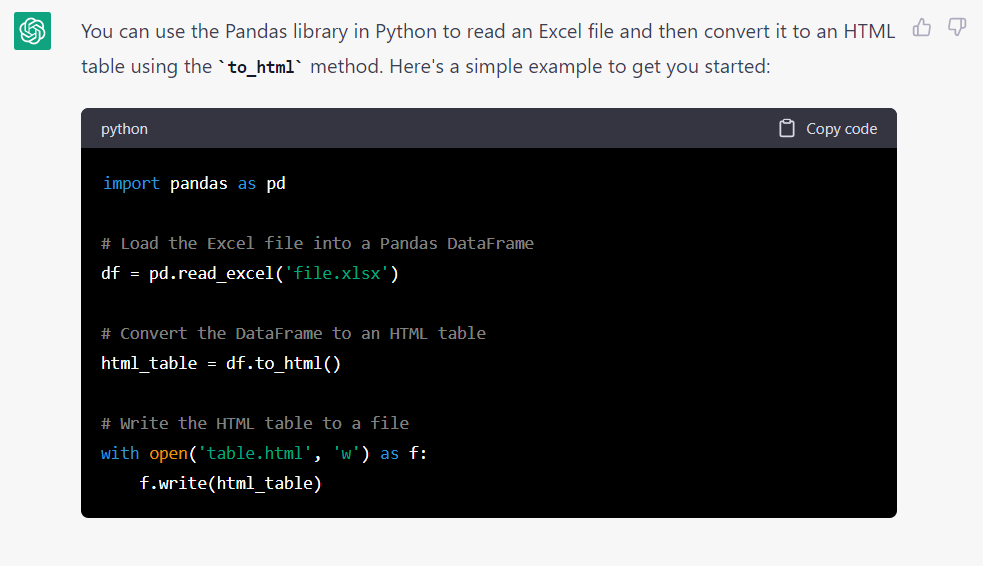
\includegraphics{ghtop_images/chatgpt_1.png}

\hypertarget{what-does-chatgpt-say-without-pandas}{%
\subsection{What does chatgpt say without
pandas?}\label{what-does-chatgpt-say-without-pandas}}

\begin{quote}
convert excel file to html in python without pandas include the excel
formatting such as column width
\end{quote}

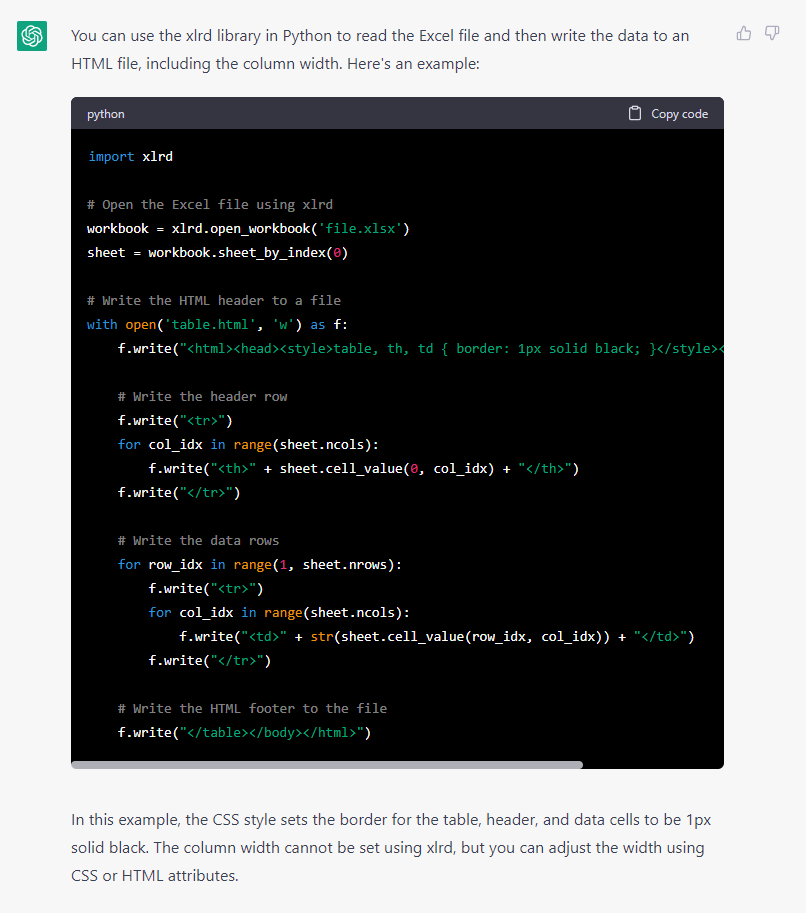
\includegraphics{ghtop_images/chatgpt_2.png}

\begin{Shaded}
\begin{Highlighting}[]
\ImportTok{import}\NormalTok{ pandas }\ImportTok{as}\NormalTok{ pd}

\ImportTok{import}\NormalTok{ os}
\ImportTok{from}\NormalTok{ pathlib }\ImportTok{import}\NormalTok{ Path}
\ImportTok{import}\NormalTok{ sys}

\NormalTok{module\_path }\OperatorTok{=}\NormalTok{ Path( os.getcwd() )}
\NormalTok{module\_path }\OperatorTok{=}\NormalTok{ module\_path.parent.parent.parent.}\FunctionTok{\_\_str\_\_}\NormalTok{() }\OperatorTok{+} \StringTok{\textquotesingle{}}\CharTok{\textbackslash{}\textbackslash{}}\StringTok{Pesticide\textquotesingle{}}

\NormalTok{cwd }\OperatorTok{=}\NormalTok{ module\_path}

\NormalTok{folder\_path }\OperatorTok{=}\NormalTok{ os.path.join(cwd,}\StringTok{\textquotesingle{}data\textquotesingle{}}\NormalTok{)}

\NormalTok{sys.path.insert(}\DecValTok{0}\NormalTok{, module\_path)}

\NormalTok{df2 }\OperatorTok{=}\NormalTok{ pd.read\_csv(os.path.join(folder\_path,}\StringTok{\textquotesingle{}combined\_df.csv\textquotesingle{}}\NormalTok{) ,index\_col}\OperatorTok{=}\DecValTok{0}\NormalTok{ )}
\CommentTok{\# change data type of columns}
\NormalTok{df2[}\StringTok{\textquotesingle{}date\_of\_sampling\textquotesingle{}}\NormalTok{] }\OperatorTok{=}\NormalTok{ pd.to\_datetime(df2[}\StringTok{\textquotesingle{}date\_of\_sampling\textquotesingle{}}\NormalTok{])}
\end{Highlighting}
\end{Shaded}

\hypertarget{pandas}{%
\subsection{pandas}\label{pandas}}

\begin{itemize}
\tightlist
\item
  Since (in Python) we are mainly working with pandas. Let's consider
  how pandas outputs can be modified.
\item
  \href{https://pandas.pydata.org/docs/user_guide/options.html}{pandas
  options}
\end{itemize}

Some code functionality

\begin{verbatim}
# precision of all columns
pd.set_option("display.precision", 2)
# Or map as a string
df2['amount_pc_str'] = df2['amount_pc'].map(lambda x: '%.3f' % x)
# some other options
pd.set_option('max_colwidth', 20)
pd.set_option('display.max_columns', None)
pd.set_option('display.expand_frame_repr', False)
pd.set_option('max_colwidth', 0)
\end{verbatim}

\hypertarget{pandas-basic}{%
\subsection{pandas basic}\label{pandas-basic}}

\begin{Shaded}
\begin{Highlighting}[]
\NormalTok{df2}
\end{Highlighting}
\end{Shaded}

\begin{longtable}[]{@{}llllllllllllllllll@{}}
\toprule()
& sample\_id & date\_of\_sampling & description & country\_of\_origin &
retail\_outlet & address & brand\_name &
packer\_/\_manufacturer\_/\_importer & product & address\_postcode &
packer\_postcode & address\_area & packer\_area & chem\_name &
amount\_detected & mrl & amount\_pc \\
\midrule()
\endhead
0 & 1958/2016 & 2016-08-08 & Bramley Apples & UK & Asda & Creechbarrow
Road, Taunton TA1 2AN & Asda & Asda Stores Ltd Leeds, UK LS11 5AD &
Apple & TA1 2AN & LS11 5AD & Somerset & West Yorkshire & boscalid & 0.03
& 2.0 & 0.015 \\
1 & 1958/2016 & 2016-08-08 & Bramley Apples & UK & Asda & Creechbarrow
Road, Taunton TA1 2AN & Asda & Asda Stores Ltd Leeds, UK LS11 5AD &
Apple & TA1 2AN & LS11 5AD & Somerset & West Yorkshire & pyraclostrobin
& 0.01 & 0.5 & 0.020 \\
2 & 0230/2016 & 2016-08-08 & Bramley Apples & UK & Co-op & Northgate,
Louth LN11 0LT & Co-op & Co-operative Group Ltd Manchester M60 0AG &
Apple & LN11 0LT & M60 0AG & Lincolnshire & Greater Manchester &
boscalid & 0.05 & 2.0 & 0.025 \\
3 & 0230/2016 & 2016-08-08 & Bramley Apples & UK & Co-op & Northgate,
Louth LN11 0LT & Co-op & Co-operative Group Ltd Manchester M60 0AG &
Apple & LN11 0LT & M60 0AG & Lincolnshire & Greater Manchester &
flonicamid (sum) & 0.02 & 0.2 & 0.100 \\
4 & 0230/2016 & 2016-08-08 & Bramley Apples & UK & Co-op & Northgate,
Louth LN11 0LT & Co-op & Co-operative Group Ltd Manchester M60 0AG &
Apple & LN11 0LT & M60 0AG & Lincolnshire & Greater Manchester &
pyraclostrobin & 0.03 & 0.5 & 0.060 \\
... & ... & ... & ... & ... & ... & ... & ... & ... & ... & ... & ... &
... & ... & ... & ... & ... & ... \\
35155 & 2858/2020 Organic & 2020-10-20 & Organic Sweet Potatoes & Spain
& Tesco & 300 Beverley Way, New Malden KT3 4PJ & Tesco & Tesco Stores
Ltd Welwyn Garden City AL7 1GA & Sweet\_Potatoes\_Q4\_(BNA) & KT3 4PJ &
AL7 1GA & Greater London & Hertfordshire & 0 & 0.00 & 0.0 & 0.000 \\
35156 & 0562/2020 Organic & 2020-10-05 & Organic Duchy Sweet Potatoes &
Egypt & Waitrose & Mill Lane, Swindon SN1 7BX & Waitrose & Waitrose Ltd
Doncastle Road, Bracknell, Berksh... & Sweet\_Potatoes\_Q4\_(BNA) & SN1
7BX & RG12 8YA & Wiltshire & Berkshire & 0 & 0.00 & 0.0 & 0.000 \\
35157 & 0563/2020 & 2020-10-05 & Sweet Potatoes & USA & Waitrose & Mill
Lane, Swindon SN1 7BX & Waitrose & Waitrose Ltd Doncastle Road,
Bracknell, Berksh... & Sweet\_Potatoes\_Q4\_(BNA) & SN1 7BX & RG12 8YA &
Wiltshire & Berkshire & 0 & 0.00 & 0.0 & 0.000 \\
35158 & 2601/2020 & 2020-10-14 & Sweet Potatoes & USA & Waitrose &
Ossington Way, Newark NG24 1FF & Waitrose & Waitrose Ltd Doncastle Road,
Bracknell, Berksh... & Sweet\_Potatoes\_Q4\_(BNA) & NG24 1FF & RG12 8YA
& Nottinghamshire & Berkshire & 0 & 0.00 & 0.0 & 0.000 \\
35159 & 2601/2020 & 2020-10-14 & Sweet Potatoes & USA & Waitrose &
Ossington Way, Newark NG24 1FF & Waitrose & Waitrose Ltd Doncastle Road,
Bracknell, Berksh... & Sweet\_Potatoes\_Q4\_(BNA) & NG24 1FF & RG12 8YA
& Nottinghamshire & Berkshire & 0 & 0.00 & 0.0 & 0.000 \\
\bottomrule()
\end{longtable}

\hypertarget{pandas-overview}{%
\subsection{pandas overview}\label{pandas-overview}}

\begin{itemize}
\tightlist
\item
  Using pandas we can control various outputs
\item
  But these still need a format to display within
\item
  And display functionality is not easy
\end{itemize}

Or convert to a
\href{file:///C:/Users/44781/Documents/GitHub/jupyter_present/df2_500.html}{html
file}

\texttt{df2.iloc{[}:500{]}.to\_html(\textquotesingle{}df2\_500.html\textquotesingle{})}

But using a style sheet as shown in
\href{https://stackoverflow.com/questions/50807744/apply-css-class-to-pandas-dataframe-using-to-html}{stack
overflow by Parfait}

\begin{Shaded}
\begin{Highlighting}[]
\NormalTok{df\_out }\OperatorTok{=}\NormalTok{ df2.iloc[:}\DecValTok{500}\NormalTok{].copy()}

\NormalTok{pd.set\_option(}\StringTok{\textquotesingle{}colheader\_justify\textquotesingle{}}\NormalTok{, }\StringTok{\textquotesingle{}center\textquotesingle{}}\NormalTok{)   }\CommentTok{\# FOR TABLE \textless{}th\textgreater{}}

\NormalTok{html\_string }\OperatorTok{=} \StringTok{\textquotesingle{}\textquotesingle{}\textquotesingle{}}
\StringTok{\textless{}html\textgreater{}}
\StringTok{  \textless{}head\textgreater{}\textless{}title\textgreater{}HTML Pandas Dataframe with CSS\textless{}/title\textgreater{}\textless{}/head\textgreater{}}
\StringTok{  \textless{}link rel="stylesheet" type="text/css" href="df\_style.css"/\textgreater{}}
\StringTok{  \textless{}body\textgreater{}}
\StringTok{    }\SpecialCharTok{\{table\}}
\StringTok{  \textless{}/body\textgreater{}}
\StringTok{\textless{}/html\textgreater{}.}
\StringTok{\textquotesingle{}\textquotesingle{}\textquotesingle{}}

\CommentTok{\# OUTPUT AN HTML FILE}
\ControlFlowTok{with} \BuiltInTok{open}\NormalTok{(}\StringTok{\textquotesingle{}df2\_500.html\textquotesingle{}}\NormalTok{, }\StringTok{\textquotesingle{}w\textquotesingle{}}\NormalTok{) }\ImportTok{as}\NormalTok{ f:}
\NormalTok{    f.write(html\_string.}\BuiltInTok{format}\NormalTok{(table}\OperatorTok{=}\NormalTok{df\_out.to\_html(classes}\OperatorTok{=}\StringTok{\textquotesingle{}mystyle\textquotesingle{}}\NormalTok{)))}
\end{Highlighting}
\end{Shaded}

\hypertarget{ipydatagrid}{%
\subsection{ipydatagrid}\label{ipydatagrid}}

https://github.com/bloomberg/ipydatagrid

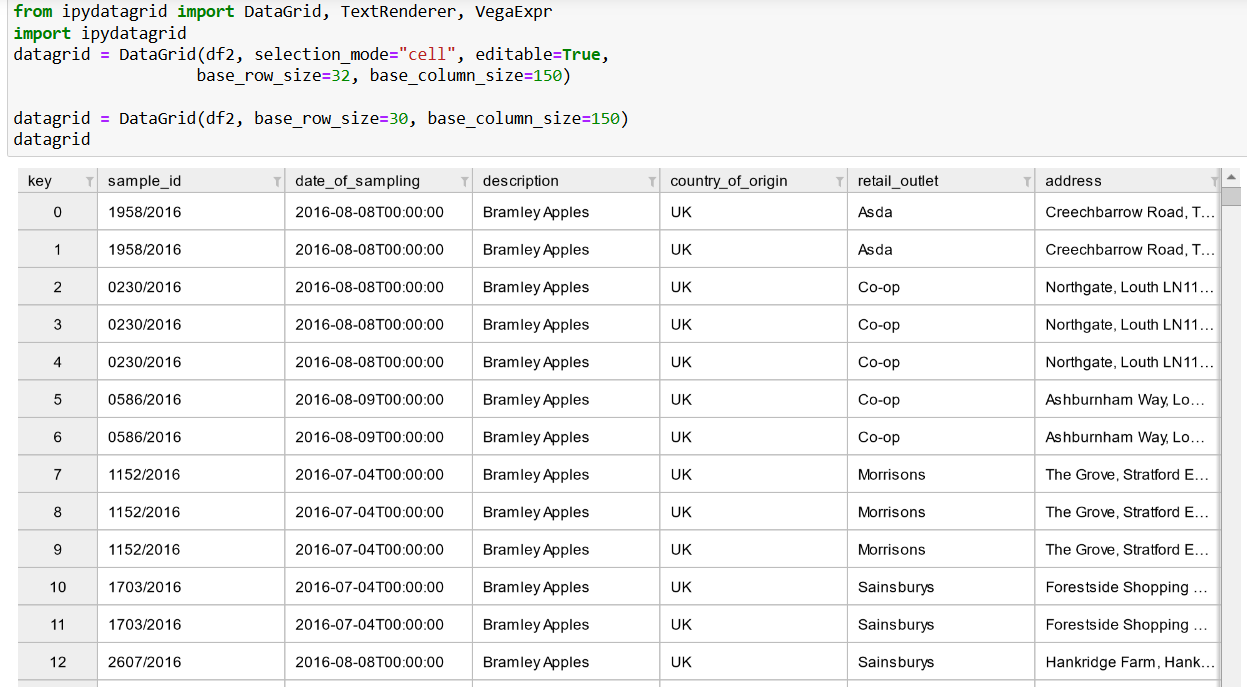
\includegraphics{ghtop_images/ipydatagrid.png}

\begin{Shaded}
\begin{Highlighting}[]
\ImportTok{from}\NormalTok{ ipydatagrid }\ImportTok{import}\NormalTok{ DataGrid, TextRenderer, VegaExpr}
\ImportTok{import}\NormalTok{ ipydatagrid}
\NormalTok{datagrid }\OperatorTok{=}\NormalTok{ DataGrid(df2, selection\_mode}\OperatorTok{=}\StringTok{"cell"}\NormalTok{, editable}\OperatorTok{=}\VariableTok{True}\NormalTok{,}
\NormalTok{                   base\_row\_size}\OperatorTok{=}\DecValTok{32}\NormalTok{, base\_column\_size}\OperatorTok{=}\DecValTok{150}\NormalTok{)}

\NormalTok{datagrid }\OperatorTok{=}\NormalTok{ DataGrid(df2, base\_row\_size}\OperatorTok{=}\DecValTok{30}\NormalTok{, base\_column\_size}\OperatorTok{=}\DecValTok{150}\NormalTok{)}
\NormalTok{datagrid}
\end{Highlighting}
\end{Shaded}

\begin{verbatim}
DataGrid(auto_fit_params={'area': 'all', 'padding': 30, 'numCols': None}, base_column_size=150, base_row_size=…
\end{verbatim}

\hypertarget{itables-code}{%
\subsection{itables code}\label{itables-code}}

\begin{verbatim}
from itables import init_notebook_mode

import itables
init_notebook_mode(all_interactive=True)

itables.show(df2)
\end{verbatim}

\begin{Shaded}
\begin{Highlighting}[]
\ImportTok{from}\NormalTok{ itables }\ImportTok{import}\NormalTok{ init\_notebook\_mode}

\ImportTok{import}\NormalTok{ itables}
\NormalTok{init\_notebook\_mode(all\_interactive}\OperatorTok{=}\VariableTok{True}\NormalTok{)}

\NormalTok{itables.show(df2)}
\end{Highlighting}
\end{Shaded}

\begin{verbatim}
<IPython.core.display.Javascript object>
\end{verbatim}

\begin{verbatim}
<IPython.core.display.HTML object>
\end{verbatim}

\begin{verbatim}
<IPython.core.display.HTML object>
\end{verbatim}

\begin{longtable}[]{@{}llllllllllllllllll@{}}
\caption{}\label{7ebb71c9-dcec-4039-a975-778753543f84}\tabularnewline
\toprule()
& sample\_id & date\_of\_sampling & description & country\_of\_origin &
retail\_outlet & address & brand\_name &
packer\_/\_manufacturer\_/\_importer & product & address\_postcode &
packer\_postcode & address\_area & packer\_area & chem\_name &
amount\_detected & mrl & amount\_pc \\
\midrule()
\endfirsthead
\toprule()
& sample\_id & date\_of\_sampling & description & country\_of\_origin &
retail\_outlet & address & brand\_name &
packer\_/\_manufacturer\_/\_importer & product & address\_postcode &
packer\_postcode & address\_area & packer\_area & chem\_name &
amount\_detected & mrl & amount\_pc \\
\midrule()
\endhead
Loading... (need
\href{https://mwouts.github.io/itables/troubleshooting.html}{help}?) & &
& & & & & & & & & & & & & & & \\
\bottomrule()
\end{longtable}

\hypertarget{dash}{%
\subsection{Dash}\label{dash}}

https://dash.plotly.com/datatable

\begin{quote}
Downloaded 800,000 times per month, Dash is the original low-code
framework for rapidly building data apps in Python, R, Julia, and F\#
(experimental).
\end{quote}

\href{Jupyter\%20dash\%20medium\%20article}{https://medium.com/plotly/introducing-jupyterdash-811f1f57c02e}

\begin{Shaded}
\begin{Highlighting}[]
\ImportTok{import}\NormalTok{ plotly.express }\ImportTok{as}\NormalTok{ px}
\ImportTok{from}\NormalTok{ jupyter\_dash }\ImportTok{import}\NormalTok{ JupyterDash}
\ImportTok{import}\NormalTok{ dash\_core\_components }\ImportTok{as}\NormalTok{ dcc}
\ImportTok{import}\NormalTok{ dash\_html\_components }\ImportTok{as}\NormalTok{ html}
\ImportTok{from}\NormalTok{ dash.dependencies }\ImportTok{import}\NormalTok{ Input, Output}\CommentTok{\# Load Data}
\NormalTok{df }\OperatorTok{=}\NormalTok{ px.data.tips()}\CommentTok{\# Build App}
\NormalTok{app }\OperatorTok{=}\NormalTok{ JupyterDash(}\VariableTok{\_\_name\_\_}\NormalTok{)}
\NormalTok{app.layout }\OperatorTok{=}\NormalTok{ html.Div([}
\NormalTok{    html.H1(}\StringTok{"JupyterDash Demo"}\NormalTok{),}
\NormalTok{    dcc.Graph(}\BuiltInTok{id}\OperatorTok{=}\StringTok{\textquotesingle{}graph\textquotesingle{}}\NormalTok{),}
\NormalTok{    html.Label([}
        \StringTok{"colorscale"}\NormalTok{,}
\NormalTok{        dcc.Dropdown(}
            \BuiltInTok{id}\OperatorTok{=}\StringTok{\textquotesingle{}colorscale{-}dropdown\textquotesingle{}}\NormalTok{, clearable}\OperatorTok{=}\VariableTok{False}\NormalTok{,}
\NormalTok{            value}\OperatorTok{=}\StringTok{\textquotesingle{}plasma\textquotesingle{}}\NormalTok{, options}\OperatorTok{=}\NormalTok{[}
\NormalTok{                \{}\StringTok{\textquotesingle{}label\textquotesingle{}}\NormalTok{: c, }\StringTok{\textquotesingle{}value\textquotesingle{}}\NormalTok{: c\}}
                \ControlFlowTok{for}\NormalTok{ c }\KeywordTok{in}\NormalTok{ px.colors.named\_colorscales()}
\NormalTok{            ])}
\NormalTok{    ]),}
\NormalTok{])}\CommentTok{\# Define callback to update graph}
\AttributeTok{@app.callback}\NormalTok{(}
\NormalTok{    Output(}\StringTok{\textquotesingle{}graph\textquotesingle{}}\NormalTok{, }\StringTok{\textquotesingle{}figure\textquotesingle{}}\NormalTok{),}
\NormalTok{    [Input(}\StringTok{"colorscale{-}dropdown"}\NormalTok{, }\StringTok{"value"}\NormalTok{)]}
\NormalTok{)}
\KeywordTok{def}\NormalTok{ update\_figure(colorscale):}
    \ControlFlowTok{return}\NormalTok{ px.scatter(}
\NormalTok{        df, x}\OperatorTok{=}\StringTok{"total\_bill"}\NormalTok{, y}\OperatorTok{=}\StringTok{"tip"}\NormalTok{, color}\OperatorTok{=}\StringTok{"size"}\NormalTok{,}
\NormalTok{        color\_continuous\_scale}\OperatorTok{=}\NormalTok{colorscale,}
\NormalTok{        render\_mode}\OperatorTok{=}\StringTok{"webgl"}\NormalTok{, title}\OperatorTok{=}\StringTok{"Tips"}
\NormalTok{    )}\CommentTok{\# Run app and display result inline in the notebook}
\NormalTok{app.run\_server(mode}\OperatorTok{=}\StringTok{\textquotesingle{}inline\textquotesingle{}}\NormalTok{)}
\end{Highlighting}
\end{Shaded}

\begin{verbatim}
C:\Users\44781\AppData\Local\Temp\ipykernel_20024\3294666565.py:3: UserWarning: 
The dash_core_components package is deprecated. Please replace
`import dash_core_components as dcc` with `from dash import dcc`
  import dash_core_components as dcc
C:\Users\44781\AppData\Local\Temp\ipykernel_20024\3294666565.py:4: UserWarning: 
The dash_html_components package is deprecated. Please replace
`import dash_html_components as html` with `from dash import html`
  import dash_html_components as html
\end{verbatim}

\begin{verbatim}
OSError: Address 'http://127.0.0.1:8050' already in use.
    Try passing a different port to run_server.
\end{verbatim}

\hypertarget{streamlit-1}{%
\subsection{Streamlit}\label{streamlit-1}}

\begin{quote}
A faster way to build and share data apps
\end{quote}

\begin{itemize}
\tightlist
\item
  Dash can be run within a notebook but is principally an app.
\item
  Streamlit is a similar app.
\item
  But much easier to code.
\end{itemize}

\begin{verbatim}
import pandas as pd
import streamlit as st
all_dfs = pd.read_csv("./data/combined_df.csv")
st.dataframe(all_dfs.head())
\end{verbatim}

\hypertarget{and-more}{%
\subsection{And more}\label{and-more}}

\hypertarget{datatables}{%
\subsubsection{\texorpdfstring{\href{https://datatables.net/}{DataTables}}{DataTables}}\label{datatables}}

\begin{quote}
DataTables is a plug-in for the jQuery Javascript library. It is a
highly flexible tool, built upon the foundations of progressive
enhancement, that adds all of these advanced features to any HTML table.
\end{quote}

\hypertarget{jupyter-widgets}{%
\subsubsection{\texorpdfstring{\href{https://ipywidgets.readthedocs.io/en/stable/}{Jupyter
widgets}}{Jupyter widgets}}\label{jupyter-widgets}}

If you are looking for Jupyter widgets, have a look at \emph{(taken from
https://mwouts.github.io/itables/references.html)} -
\href{https://github.com/quantopian/qgrid}{QGrid} by Quantopian -
\href{https://dgothrek.gitlab.io/ipyaggrid/}{IPyaggrid} by Louis Raison
and Olivier Borderies -
\href{https://github.com/QuantStack/ipysheet}{IPySheet} by QuantStack.



\end{document}
